\documentclass[a4paper,11pt]{jsarticle}

% 数式
\usepackage{amsmath,amsfonts}
\usepackage{amsthm}
\usepackage{bm}
\usepackage{mathtools}
\usepackage{amssymb}
\usepackage{color}

% 表
\usepackage[utf8]{inputenc}
\usepackage{diagbox} % 斜線付きセルを作成するために必要
\usepackage{booktabs} % 表の罫線を美しくするために必要
\usepackage{hhline} % 水平罫線を制御するために必要

% 画像
\usepackage[dvipdfmx]{graphicx}
\usepackage{ascmac}
\usepackage{physics}
\usepackage{float} % 追加

% 図
\usepackage[dvipdfmx]{graphicx}
\usepackage{tikz} %図を描く
\usetikzlibrary{positioning, intersections, calc, arrows.meta,math} %tikzのlibrary

% ハイパーリンク
\usepackage[dvipdfm,
  colorlinks=false,
  bookmarks=true,
  bookmarksnumbered=false,
  pdfborder={0 0 0},
  bookmarkstype=toc]{hyperref}

% 式番号を章ごとにリセット
\numberwithin{equation}{section}

\begin{document}

\title{9章}
\author{大上由人}
\date{\today}
\maketitle

\setcounter{section}{8}
\section{情報熱力学}
\subsection{Maxwellのdemon}
\subsubsection{Maxwellのdemon(1)}
Maxwellのdemonと呼ばれる思考実験について考察する。初め左右の部屋が等温である系について、粒子の測度が速いものと遅いものを区別するdemonがいるとする。このとき、demonは、粒子の速いものを一方の部屋に、遅いものをもう一方の部屋に分けることができる。
そうすると、最終的に左右の部屋の温度が異なる状態になり、系のエントロピーが減少するように思われる。
\begin{figure}[H]
    \begin{center}
    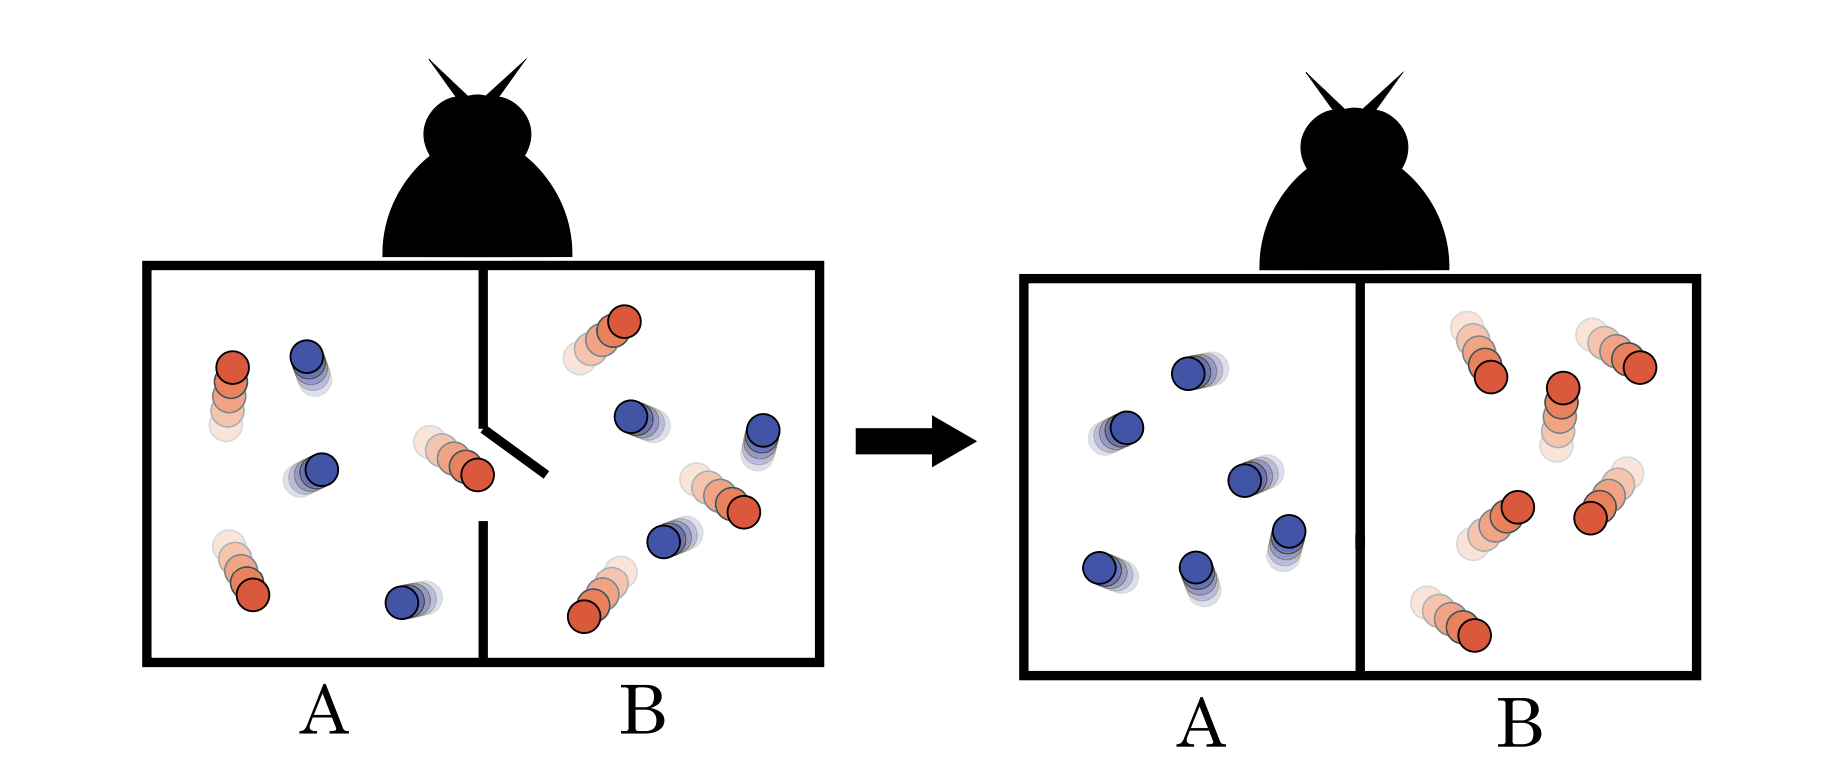
\includegraphics[width=100mm]{demon.png}
    \end{center}
    \caption{Maxwellのdemon}
    \label{fig:Maxwelldemon}
\end{figure}

\subsubsection{Szilard engine}
Maxwellのdemonを単純化したものとして、シラードエンジンとよばれる等温サイクルを考察する。シラードエンジンの過程は以下の通りである。\\
\begin{figure}[H]
    \begin{center}
    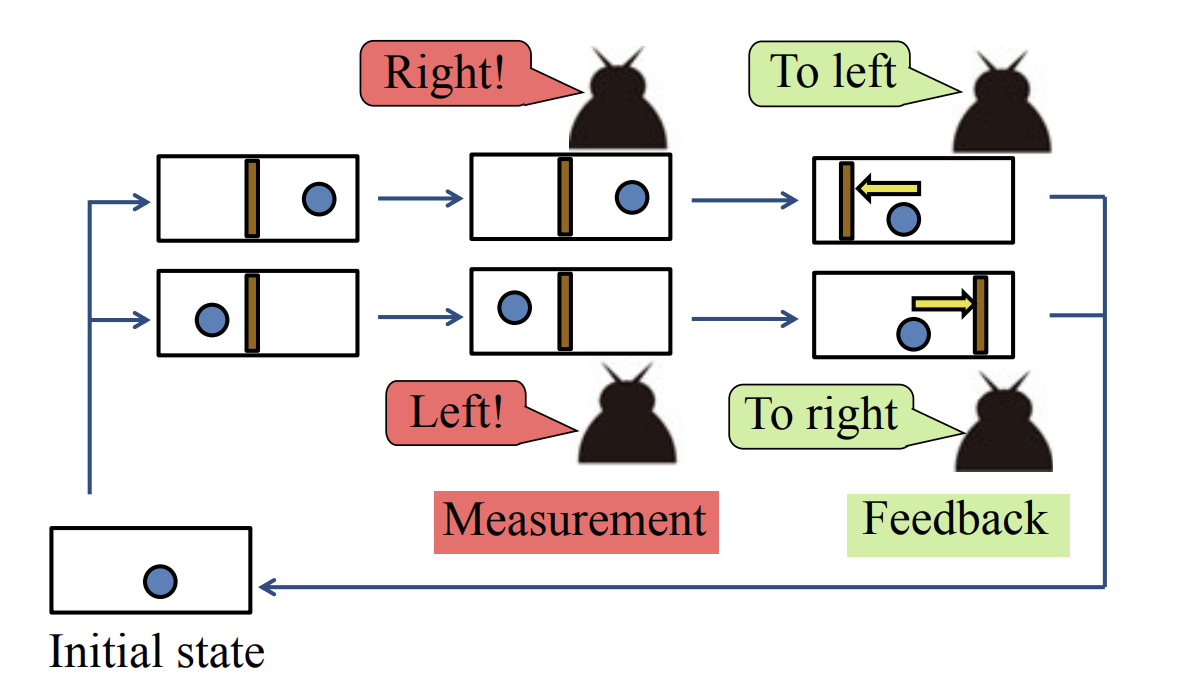
\includegraphics[width=100mm]{Szilard.png}
    \end{center}
    \caption{Szilard engine}
    \label{fig:Szilard}
\end{figure}
透熱容器の中に1粒子理想気体が入っている系(engine)をみる。系は熱浴に接している(すなわち、以下のサイクルは等温過程)。過程は以下の通りである。
\begin{enumerate}
    \item 粒子が容器全体に存在し得る状態から始める。
    \item demonが、容器にしきりを入れる。このとき、粒子は左右のどちらかに入り、demonは、粒子がどちらにいるかを確認する。(measurement)
    \item 粒子のない方向にしきりを動かす。(feedback)
    \item 壁を取り除く(初期状態に戻る)。
\end{enumerate}
このとき、3つ目の過程で仕事をとりだすことができる。とくに、容器のちょうど半分にしきりを設けるとき、この仕事は、
\begin{equation}
    W_{\text{ext}} = \int_{\frac{V}{2}}^V PdV = \int_{\frac{V}{2}}^V \frac{kT}{V}dV = kT\log 2
\end{equation}
となる。この結果は、一見すると、マクロ系の熱力学におけるKelvinの原理に反するように思える。
\footnote{
    Kelvinの原理は、任意の等温サイクルにおいて、
    \begin{equation}
        W_{\text{ext}} \leq 0
    \end{equation}
    であるという原理であった。
}
Szilardは、測定過程を熱機関と測定装置を相関付ける過程と考え、feedback過程をその相関を消費するものとして考えた。それを踏まえて、熱力学第二法則に反しないためには、
測定によるエントロピー生成が以下の不等式を満たす必要があると考えた:
\begin{equation}
    e^{-\frac{\bar{S_1}}{k}} + e^{-\frac{\bar{S_2}}{k}} \leq 1 \label{eq:9.1}
\end{equation}
ここで、$\bar{S_1}$は、粒子が領域1にいるときの平均エントロピー生成、$\bar{S_2}$は、粒子が領域2にいるときの平均エントロピー生成である。\\
\textbf{(\ref{eq:9.1})式の導出}\\
$p_i = \frac{V_i}{V}$を粒子が領域iにいる確率とする。初め、粒子は容器の全体に存在し得るので、エントロピーは
\begin{align}
k\log V + \text{const.}
\end{align}
である。同様に粒子が領域1,2にいるときのエントロピーは、それぞれ、
\begin{align}
    S_1 &= k\log V_1 + \text{const.} \\
    S_2 &= k\log V_2 + \text{const.}
\end{align}
である。よって、系の平均エントロピー変化は、
\begin{align}
    \bar{s} &=p_1k(\log V_1 - \log V) + p_2k(\log V_2 - \log V) \\
    &= k(p_1\log p_1 + p_2\log p_2)
\end{align}
となる。また、測定過程において、粒子が領域1,2にいるときの相関付けによるエントロピー生成をそれぞれ$\bar{S_1},\bar{S_2}$とすると、その平均は、
\begin{align}
    \bar{S} = p_1\bar{S_1} + p_2\bar{S_2}
\end{align}
である。全系についての熱力学第二法則は、
\begin{align}
    \bar{S} + \bar{s} &= p_1\bar{S_1} + p_2\bar{S_2} + k(p_1\log p_1 + p_2\log p_2) \geq 0
\end{align}
である。ここで、左辺を最小化することを考える。これは、ラグランジュの未定乗数法を用いて、
\begin{align}
    p_1\bar{S_1} + p_2\bar{S_2} + k(p_1\log p_1 + p_2\log p_2) + k\lambda(1-p_1-p_2)
\end{align}
を最小化することと等価である。$p_1,p_2,\lambda$についてそれぞれ偏微分すると、
\begin{align}
    &\bar{S_1} +k\log p_1 - k + k\lambda = 0 \\
    &\bar{S_2} +k\log p_2 - k + k\lambda = 0 \\
    &1-p_1-p_2 = 0
\end{align}
となる。これを変形して、
\begin{align}
    p_1 &= \exp(\lambda - \frac{\bar{S_1}}{k}) \\
    p_2 &= \exp(\lambda - \frac{\bar{S_2}}{k})
\end{align}
となる。これを用いて、
\begin{align}
    \lambda e^{\lambda}(e^{-\frac{\bar{S_1}}{k}} + e^{-\frac{\bar{S_2}}{k}}) \geq 0
\end{align}
となる。これより$\lambda \geq 0$であることがわかる。ここで、
\begin{align}
    p_1 + p_2 &= \exp(\lambda - \frac{\bar{S_1}}{k}) + \exp(\lambda - \frac{\bar{S_2}}{k}) = 1
\end{align}
より、
\begin{align}
    e^{-\frac{\bar{S_1}}{k}} + e^{-\frac{\bar{S_2}}{k}}  = e^{-\lambda} \leq 1
\end{align}
となる。よって、(\ref{eq:9.1})式が導かれる。\hfill\qedsymbol\\

\textbf{具体的なメモリーの導入}\\
Szilardは、(\ref{eq:9.1})式を満たすようなメモリーも導入した。以下ではその概要を見る。\\

\begin{figure}[H]
    \centering
\begin{tikzpicture}
    % Drawing the energy levels
    \draw[thick] (0,0) -- (1,0);
    \draw[thick] (0,2) -- (1,2);
    \draw[thick] (1.5,2) -- (2.5,2);
    \draw[thick,dotted] (3,2) -- (4,2);
    \draw[thick] (4.5,2) -- (5.5,2);
    
    % Label for degenerate levels
    \node at (2.5,2.5) {$g$個};
    \node at (-0.5,2) {$B$};
    \node at (-0.5,0) {$A$};
    
    % Energy axis
    \draw[->] (6.1,0) -- (6.1,3) node[anchor=west] {E};
    \draw (6.1,0) -- (5.9,0) node[anchor=east] {0};
    \draw (6.1,2) -- (5.9,2) node[anchor=east] {u};
\end{tikzpicture}
\caption{メモリーのエネルギー準位}
\label{fig:memory}
\end{figure}
図\ref{fig:memory}のような系を考える。1つのエネルギー準位が0であり、他のg個のエネルギー準位がuであるとする。エネルギーが低い準位、高い準位をそれぞれA,Bとする。
初期状態における温度を$T_0$とする。系の状態が$x =1,2$のとき、メモリーの温度を$T_A,T_B$とする。ただし、$T_A <T_0<T_B$であるとする。\\
このとき、メモリーの平均エネルギーは、
\begin{align}
    \bar{u}(T) = uq(T) = \frac{uge^{-\frac{u}{kT}}}{1+ge^{-\frac{u}{kT}}}
\end{align}
である。このとき、測定によるエントロピー生成とメモリー消去によるエントロピー生成の合計は、
\begin{align}
    S_i = \frac{\bar{u}(T_i)-\bar{u}(T_0)}{T_0} + \int_{T_i}^{T_0}\frac{1}{T}\frac{\dd \bar{u}(T)}{\dd T}\dd T
\end{align}
である。第一項がメモリー消去、第二項が測定によるエントロピー生成である。これを整理すると、%TODO: ここから先を書く
\begin{align}
    S_i = k\left(q(T_i)\log\frac{q(T_i)}{q(T_0)} + p(T_i)\log\frac{p(T_i)}{p(T_0)}\right) \label{eq:a}
\end{align}
となる。ただし、
\begin{align}
    p(T) &= \frac{1}{1+ge^{-\frac{u}{kT}}} \\
    q(T) &= \frac{ge^{-\frac{u}{kT}}}{1+ge^{-\frac{u}{kT}}}
\end{align}
である。\\
\textbf{(\ref{eq:a}式の導出)}\\
\begin{align}
    S_i &= \frac{\bar{u}(T_i)-\bar{u}(T_0)}{T_0} + \int_{T_i}^{T_0}\frac{1}{T}\frac{\dd \bar{u}(T)}{\dd T}\dd T \\
    &= \frac{\bar{u}(T_i)-\bar{u}(T_0)}{T_0} + \int_{T_i}^{T_0}\left(\dv{T} \left(\frac{\bar{u}(T)}{T} +k\log(1+ge^{-\frac{u}{kT}})\right)\right)\dd T \\
    &= \frac{\bar{u}(T_i)-\bar{u}(T_0)}{T_0} + \left(\frac{\bar{u}(T_0)}{T_0} +k\log(1+ge^{-\frac{u}{kT_0}})\right) - \left(\frac{\bar{u}(T_i)}{T_i} +k\log(1+ge^{-\frac{u}{kT_i}})\right) \\
    &= \bar{u}(T_i)\left(\frac{1}{T_0} - \frac{1}{T_i}\right) + k\log\frac{1+ge^{-\frac{u}{kT_0}}}{1+ge^{-\frac{u}{kT_i}}} \\
    &= q(T_i)\left(\frac{u}{T_0} - \frac{u}{T_i}\right) + k\log\frac{p(T_i)}{p(T_0)} \quad \because \frac{1}{p(T)} = 1+ge^{-\frac{u}{kT}}\\
    &= q(T_i)\left(-k\log\frac{q(T_0)}{p(T_0)}\right) + k\log\frac{q(T_i)}{p(T_i)} + k\log\frac{p(T_i)}{p(T_0)} \\
    &= q(T_i)k\log\frac{p(T_0)}{q(T_0)}\frac{q(T_i)}{p(T_i)} + k\log\frac{p(T_i)}{p(T_0)} \\
    &= q(T_i)k\log\frac{q(T_i)}{q(T_0)} - q(T_i)k\log\frac{p(T_i)}{p(T_0)} + k\log\frac{p(T_i)}{p(T_0)} \\
    &= q(T_i)k\log\frac{q(T_i)}{q(T_0)} + p(T_i)k\log\frac{p(T_i)}{p(T_0)} \quad \because p(T) + q(T) = 1\\
    &= k\left(q(T_i)\log\frac{q(T_i)}{q(T_0)} + p(T_i)\log\frac{p(T_i)}{p(T_0)}\right)
\end{align}
により、(\ref{eq:9.1})式が導かれる。\footnote{
    二つ目の等号で、
    \begin{align}
        \frac{1}{T}\dv{\bar{u}(T)}{T} = \dv{T}\left(\frac{\bar{u}(T)}{T} + k\log(1+ge^{-\frac{u}{kT}})\right)
    \end{align}
    であることを用いた。これは計算により確かめることができ、
    \begin{align}
        \dv{T}\left(\frac{\bar{u}(T)}{T} + k\log(1+ge^{-\frac{u}{kT}})\right) &= \frac{1}{T}\dv{\bar{u}(T)}{T} - \frac{\bar{u}(T)}{T^2} + k\frac{ge^{-\frac{u}{kT}}}{1+ge^{-\frac{u}{kT}}}\left(\frac{u}{kT^2}\right) \\
        &= \frac{1}{T}\dv{\bar{u}(T)}{T} -q(T)\frac{u}{T^2} +kq(T)\frac{u}{kT^2} \\
        &= \frac{1}{T}\dv{\bar{u}(T)}{T} 
    \end{align}
    であることがわかる。教科書(9.11)式は誤植っぽい。
}\hfill\qedsymbol\\

これの極限を考える。$T_A \to 0,g \to \infty$とすると、$p(T_A) = q(T_B) = 1, p(T_B) = q(T_A) = 0$となる。よって、
\begin{align}
    & S_A = -k\log p(T_0) \\
    & S_B = -k\log q(T_0)
\end{align}
となる。これは、(\ref{eq:9.1})式の等号が成り立つときのエントロピー生成である。\\

\subsubsection{BrillouinとGaborの議論}
Brillouin、Gaborの議論についてみる。\\
Brillouinは、光を用いて粒子の位置を測定することを考えた。光が粒子に当たると光が散乱し、そのエネルギーが熱に変わる。測定結果を見るには$h\nu \gg kT$である必要がある。(背景輻射との区別をするため。)
このとき、測定過程におけるエントロピーが、feedback過程で取り出される仕事よりも大きくなるため、熱力学第二法則に反しないと考えた。\\

また、Gaborも光を用いて粒子の位置を測定することを考えた。
箱の中に単一の粒子が入っている。ある$X>1$を固定し、粒子が箱の底の$\frac{1}{X}$の範囲にいるかどうかを考える。粒子がこの領域の中に入っていたら、箱の底と上側とを分離する壁を挿入する。
壁が挿入されると、粒子のエントロピーは$kT\log X$だけ減少する。Gaborは、この測定には少なくとも$\frac{X}{2}$個の光子が必要であると考えた。このとき、$\frac{Xh\nu}{2} $以上のエネルギーが散乱される(これは、エントロピーによる利得$kT\log X$よりもはるかに大きい)。\\

\subsubsection{LandauerとBennettの議論}
LandauerおよびBennettの議論についてみる。彼らは、メモリー消去にかかるコストに注目した。\\

\begin{figure}
    \begin{center}
    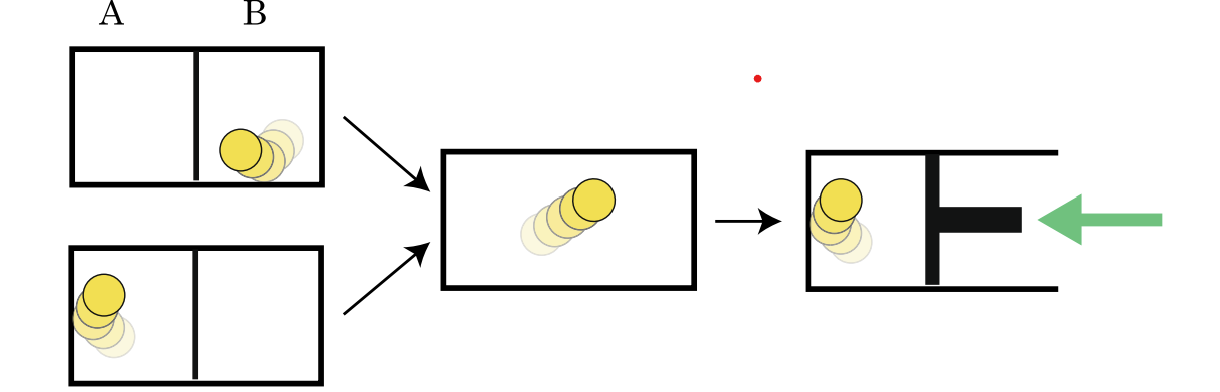
\includegraphics[width=100mm]{Landauer.png}
    \end{center}
    \caption{Landauerの原理}
    \label{fig:Landauer}
\end{figure}

メモリー消去は、消去前の状態によらず、一意な状態になる。このとき、シャノンエントロピーが減少する。このシャノンエントロピーの減少が、熱放出と結びついていると考えた(Landauerの原理)。\\

Bennettもmemory消去にかかるコストに注目した。彼は以下のような具体例を構成した。\\
\begin{figure}[H]
    \begin{center}
    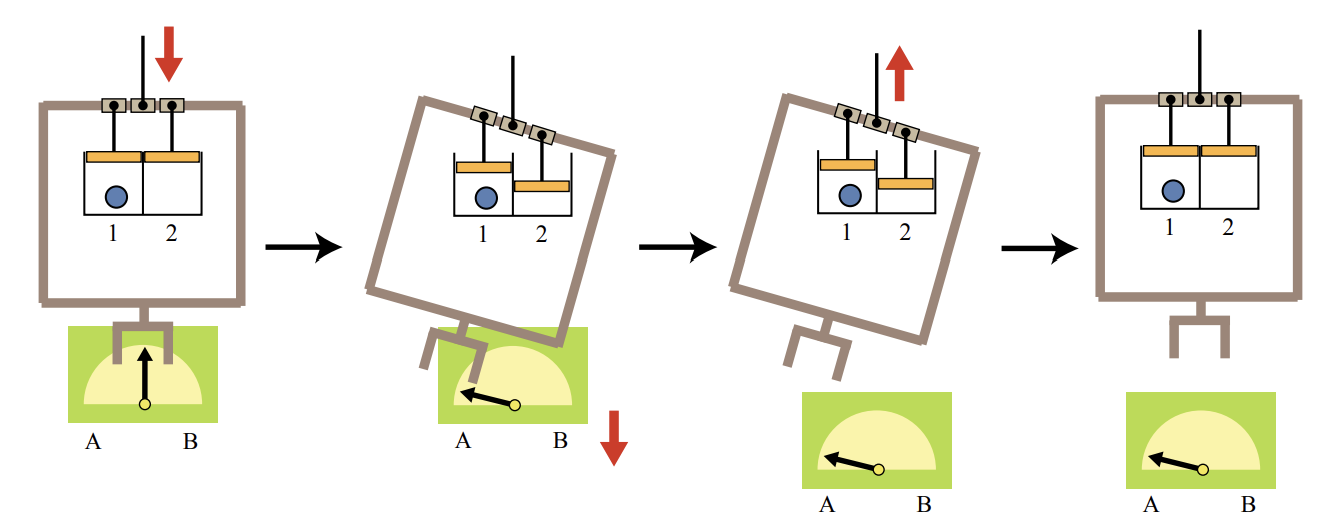
\includegraphics[width=100mm]{Bennett.png}
    \end{center}
    \caption{Bennettの議論}
    \label{fig:Bennett}
\end{figure}
\begin{enumerate}
    \item ピストンを準静的に下げ、engineの状態を記録する。(この過程では仕事が必要)
    \item メモリー消去を行い、ピストンを準静的に上げる。(この過程では、一つ前と同じだけの仕事を取り出すことができる)
\end{enumerate}
これはBrillouinの議論の反例である。\\

\subsubsection{Maxwell demonは解決されたか}
Maxwell demonの問題は、engineとmemoryの相関が大事であり、メモリー消去が大事なわけではないということを言っている。

\subsection{情報熱力学の第二法則}
\subsubsection{相互情報量}
二つの確率変数の相関を測る指標として、相互情報量を導入する。\\
\begin{itembox}[l]{\textbf{Def:相互情報量}}
    二つの確率変数$x,y$について、その相互情報量$I(x,y)$は、
    \begin{align}
        I(x,y) = \sum_{i,j}P(x_i,y_j)\log\frac{P(x_i,y_j)}{P(x_i)P(y_j)}
    \end{align}
    で定義される.

\end{itembox}
このとき、シャノンエントロピーの定義と見比べることで、
\begin{align}
    I(x,y) = H(x) - H(x|y) = H(y) - H(y|x)
\end{align}
であることがわかる。\\%TODO: ここの計算しておく
$(\because$)\\
定義から、
\begin{align}
    H(x|y) &= -\sum_{i,j}P(x_i,y_j)\log P(x_i|y_j) \\
    H(x) &= -\sum_{i}P(x_i)\log P(x_i)
\end{align}
である。よって、
\begin{align}
    I(x,y) &= \sum_{i,j}P(x_i,y_j)\log\frac{P(x_i,y_j)}{P(x_i)P(y_j)} \\
    &= \sum_{i,j}P(x_i,y_j)\log \frac{P(x_i|y_j)P(y_j)}{P(x_i)P(y_j)} \\
    &= \sum_{i,j}P(x_i,y_j)\log \frac{P(x_i|y_j)}{P(x_i)} \\
    &= \sum_{i,j}P(x_i,y_j)\log \frac{P(x_i,y_j)}{P(x_i)} \\
    &= H(x) - H(x|y)
\end{align}
である。\hfill\qedsymbol\\
この式を見ると、相互情報量は、$y$の値を知ることによる、エントロピーの減少量と解釈することができる。\\
今、
\begin{align}
    I(x,y) = H(x) - H(x|y) \geq 0
\end{align}
であるから、相互情報量は、常に非負である。とくに、$x,y$が独立であるとき、
\begin{align}
    I(x,y) = 0
\end{align}
である。これは、$y$の値を知っても、$x$の値に関する情報が何も得られないことに対応している。\\

また、確率的な相互情報量も導入しておく。
\begin{itembox}[l]{\textbf{Def:確率的相互情報量}}
        確率的相互情報量$\hat{I}(x,y)$は、
        \begin{align}
                \hat{I}(x,y) = \log\frac{P(x,y)}{P(x)P(y)}
        \end{align}
        で定義される.

\end{itembox}
確率的相互情報量の期待値は、相互情報量と等しい。\\

\subsubsection{情報熱力学の第二法則}
$X$と$Y$の複合系を考える。この節では、$X$のみが、$Y$に依存して時間発展することができ、$Y$は時間発展しないとする。
初め、$X$と$Y$は相関があってもよいとする。\\
初期状態及び終状態の相互情報量を、$I_{\text{i}},I_{\text{f}}$とする。また、初期状態および終状態の系$X,Y$のエントロピーを、それぞれ、$S_{X\text{i}},S_{Y\text{i}},S_{X\text{f}},S_{Y\text{f}}$とする。\\
このとき、初期状態及び終状態の全系のシャノンエントロピーは、
\begin{align}
    S_{\text{tot,i}} &= S_{X\text{i}} + S_{Y\text{i}} - I_{\text{i}} \\
    S_{\text{tot,f}} &= S_{X\text{f}} + S_{Y\text{f}} - I_{\text{f}}
\end{align}
である。\\
%TODO: ここの計算をする
$(\because)$\\
相互情報量の定義から、
\begin{align}
    I_{\text{i}} &= \sum_{i,j}P_{\text{i}}(x_i,y_j)\log\frac{P_{\text{i}}(x_i,y_j)}{P_{\text{i}}(x_i)P_{\text{i}}(y_j)} \\
    &= \sum_{i,j}P_{\text{i}}(x_i,y_j)\log P_{\text{i}}(x_i,y_j) - \sum_{i,j}P_{\text{i}}(x_i,y_j)\log P_{\text{i}}(x_i) - \sum_{i,j}P_{\text{i}}(x_i,y_j)\log P_{\text{i}}(y_j) \\
    &= -S_{X\text{tot,i}}  + S_{X\text{i}} + S_{Y\text{i}}
\end{align}
である。終状態についても同様である。\hfill\qedsymbol\\


このとき、全系についての熱力学第二法則は、
\begin{align}
    \sigma_X = \Delta S_X +\beta Q_X \geq \Delta I
\end{align}
である。この関係は、沙川-上田関係とも呼ばれる。(9.3で導出する)\\
この関係は、相関の強さが変わったら、(たとえ片方が時間変化しないとしても)それに合わせて熱力学第二法則を修正する必要があるということである。\\

\subsubsection{Szilardエンジン}
沙川-上田関係を用いて、シラードエンジンについて考察する。\\
\begin{figure}[H]
    \begin{center}
    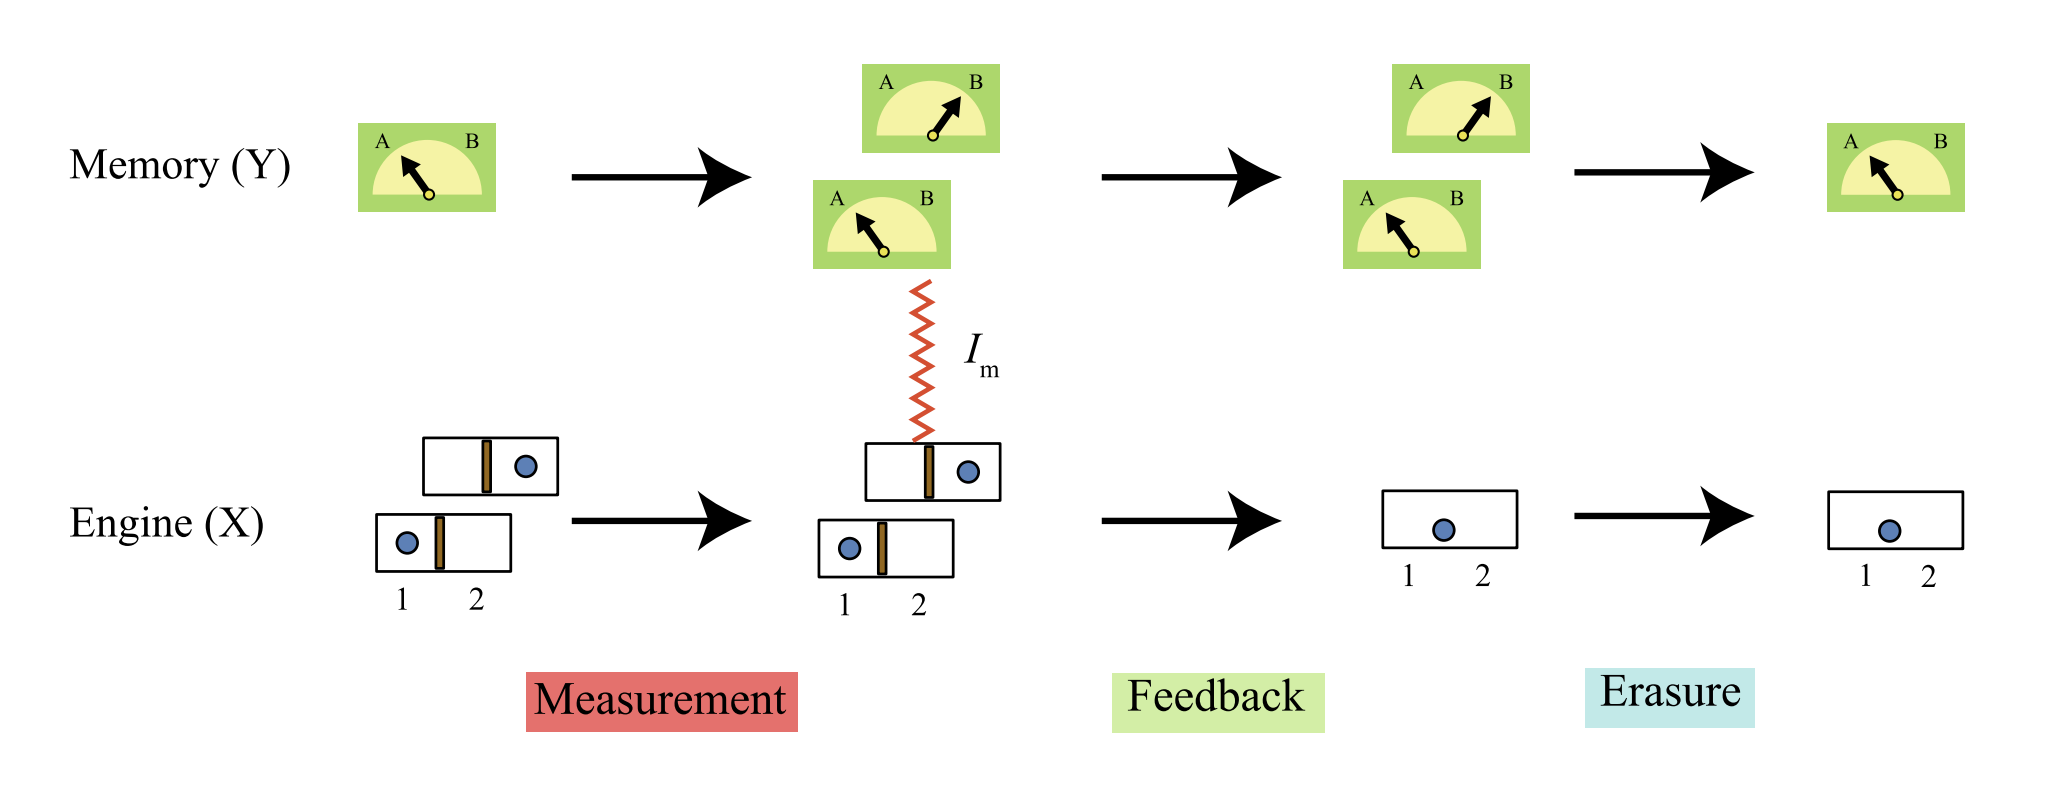
\includegraphics[width=100mm]{s.png}
    \end{center}
    \caption{Szilard engine}
    \label{fig:s}
\end{figure}

$W$を取り出されるエネルギーとして、エントロピー生成は、
\begin{align}
    \sigma = -\beta W + \Delta S
\end{align}
である。ここで、$\Delta S$は、エントロピーの変化である。また、測定過程のあとの相互情報を$I_{\text{mem}}$とする。\\

\textbf{測定過程}\\
しきりを入れたときに、AまたはBのどちらかに粒子が入り、メモリーのシャノンエントロピーが増加する。また、engineとメモリーの間に相関ができる。このときの沙川-上田関係は、engineが時間変化しないとして、
\begin{align}
    \ev{e^{-\hat{\sigma}_Y+\hat{I}_{\text{mem}}}} = 1
\end{align}
すなわち、
\begin{align}
    \sigma_Y \geq I_{\text{mem}}
\end{align}
である。\\

\textbf{feedback過程}\\
情報量が変わらないため、engineのエントロピーは変化しないのに対し、しきりを動かすため、外部に仕事を取り出すことができる。また、engineとメモリーが相関を失う。このときの沙川-上田関係は、memoryが時間変化しないとして、

\begin{align}
    \ev{e^{-\hat{\sigma}_X-\hat{I}_{\text{mem}}}} = 1
\end{align}
すなわち、
\begin{align}
    \sigma_X \geq -I_{\text{mem}}
\end{align}
である。\\

\textbf{メモリーの消去}\\
粒子がどちらにいたかの情報をリセットするので、その分メモリのシャノンエントロピーが減少する。また、メモリをもとの状態に戻すために外部から仕事をされる。このときの沙川-上田関係は、
\begin{align}
    \ev{e^{-\hat{\sigma}_Y}} = 1
\end{align}
すなわち、
\begin{align}
    \sigma_Y \geq 0
\end{align}
である。\\

これまでの過程をまとめると、以下の図のようになる。\\
\begin{figure}[H]
    \begin{center}
    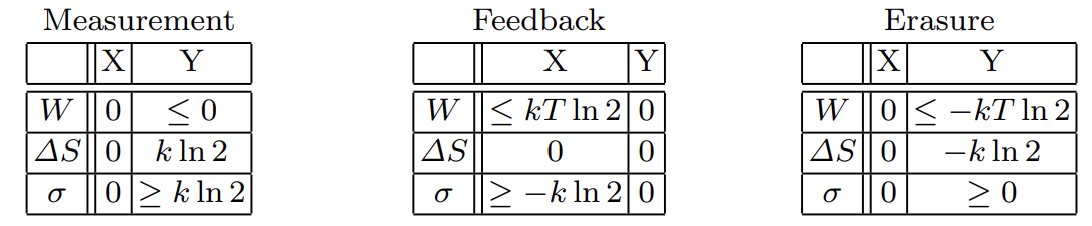
\includegraphics[width=100mm]{mfe.png}
    \end{center}
    \caption{Szilard engine}
    \label{fig:mfe}
\end{figure}
上の議論からわかるように、熱力学第二法則に修正が必要なのは、測定過程とfeedback過程である。メモリー消去の過程については、普通の熱力学と同じである。このことを踏まえると、メモリー消去を含まないようなシラードエンジンを構成することができる。

\begin{figure}[H]
    \begin{center}
    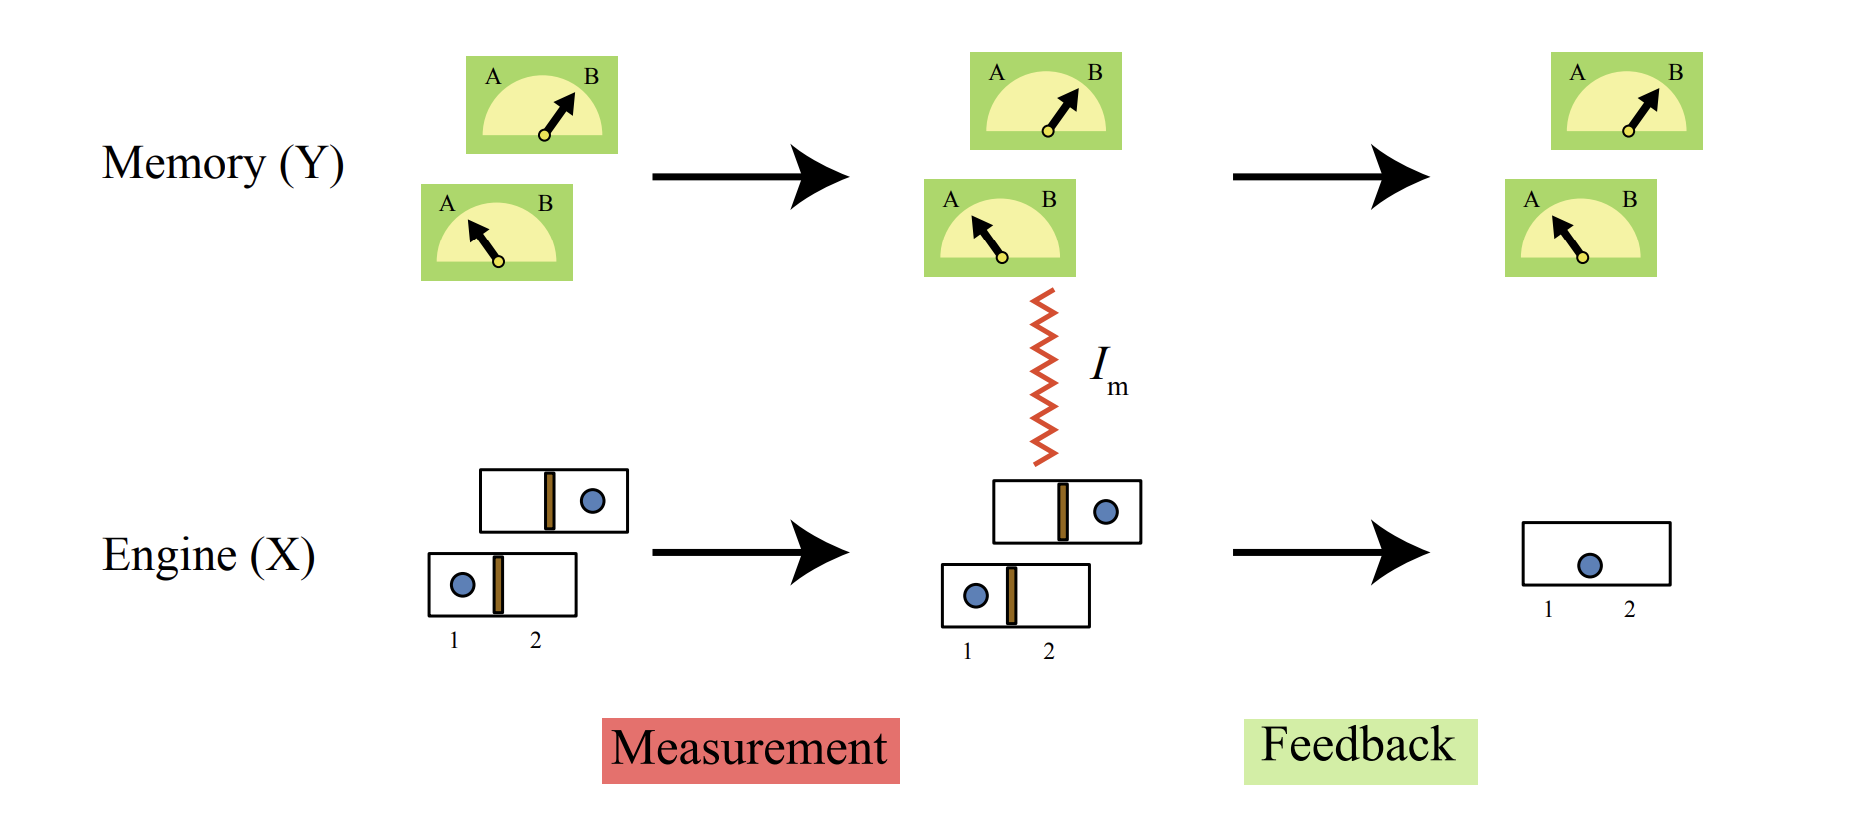
\includegraphics[width=100mm]{s2.png}
    \end{center}
    \caption{メモリー消去を含まないようなシラードエンジン}
    \label{fig:s2}
\end{figure}

普通のシラードエンジンと異なる点は、初期状態のメモリの状態を固定しない点である。この過程においては、memoryのシャノンエントロピーは変化しない(過程の間ずっとmemoryは2通りの状態をとる)。このような過程ではmemoryに仕事がなされることになる。\\
過程をまとめると、以下の図のようになる。\\
\begin{figure}[H]
    \begin{center}
    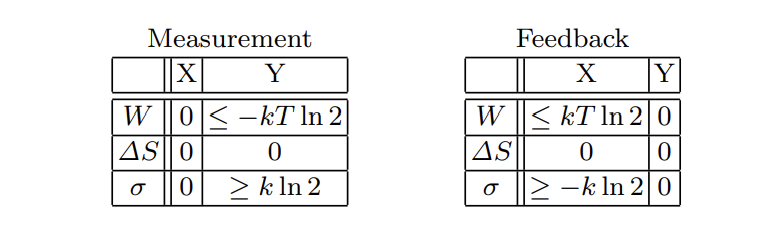
\includegraphics[width=100mm]{cycle.png}
    \end{center}
    \caption{メモリー消去を含まないようなシラードエンジン}
    \label{fig:cycle}
\end{figure}
これは、測定過程においては仕事を要することを示しており、Bennettの議論はもはや適応できないことを示している。\\

\newpage
\subsection{沙川-上田関係}
沙川-上田関係を導出する。\\
\subsubsection{沙川-上田関係の導出}
\textbf{設定}\\
\begin{figure}[H]
    \begin{center}
    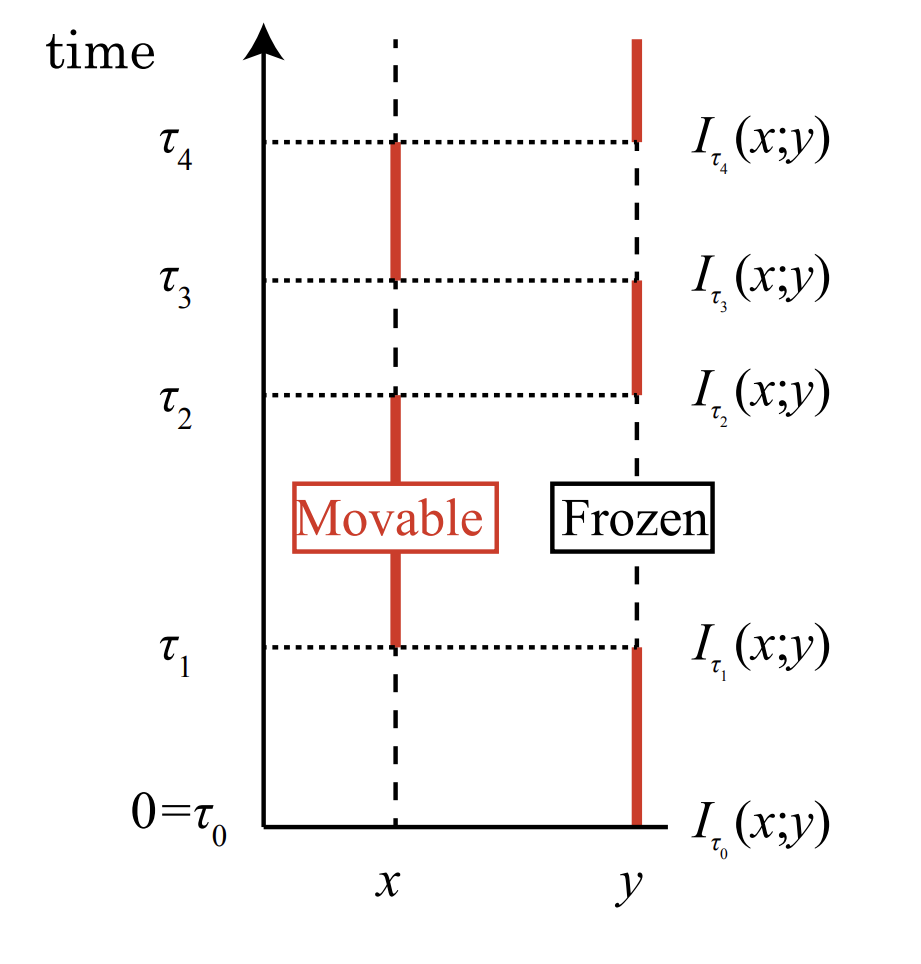
\includegraphics[width=80mm]{Sagawa.png}
    \end{center}
    \caption{Sagawa-Ueda setup}
    \label{fig:Sagawa}
\end{figure}

\begin{itemize}
    \item 時刻$0 \leq t \leq \tau$の間に、系$X$(engine)と$Y$(memory)の間で$N$回のmeasurementとfeedbackを行う。
    \item $0 \leq t \leq \tau$を$2N$個の区間に分割し、$ 0 = \tau_0 \leq \tau_1 \leq \cdots \leq \tau_{2N} = \tau$とする。
    \item $\tau_{2n} \leq t \leq \tau_{2n+1}\quad(n=0,1,\cdots,N-1)$の間は、$Y$のみ状態が変化し、measurementが行われる。
    \item $\tau_{2n+1} \leq t \leq \tau_{2n+2}\quad(n=0,1,\cdots,N-1)$の間は、$X$のみ状態が変化し、feedbackが行われる。
    \item $\tau_{2n} \leq t \leq \tau_{2n+1}$と$\tau_{2n+1} \leq t \leq \tau_{2n+2}\quad(n=0,1,\cdots,N-1)$の時間間隔をそれぞれ第$n$Y-フェーズとX-フェーズと呼ぶ。
    \item 第$n$X-フェーズについて、$m_n$をXでのジャンプ回数とし、$t_{n,i}$を第$i$回ジャンプが発生する時間とする。$t_{n,i}$でのジャンプはXの状態を$x^{n,i-1}$から$x^{n,i}$に変える。
    \item $t_{n,0} := \tau_{2n+1}$と$t_{n,m_n+1} := \tau_{2n+2}$とする。(Xに切り替わった瞬間はjumpしない)
    \item $x$は$\tau_{2n} \leq t \leq \tau_{2n+1}$の間(すなわち、Yがmovableなとき)に変化しないため、$x^{n-1,m_{n-1}} = x(\tau_{2n}) = x(\tau_{2n+1}) = x^{n,0}$が成り立つ。
    \item $y$は$\tau_{2n+1} \leq t \leq \tau_{2n+2}$の間(すなわち、Xがmovableなとき)に変化しないため、$y(\tau_{2n+1}) = y(\tau_{2n+2})$が成り立つ。
\end{itemize}

このとき、系$X$のエントロピー生成は、
\begin{align}
    \hat{\sigma}_X := \sum^{N-1}_{n=0} \sum^{m_n}_{i=1} \ln \frac{P^{x^{n,i-1} \to x^{n,i}; y(\tau_{2n+1}), t^{n,i}}}{P^{x^{n,i} \to x^{n,i-1}; y(\tau_{2n+1}), t^{n,i}}} - \ln P(x(\tau); \tau) + \ln P(x(0); 0)
\end{align}
ただし、第一項は系$X$に接触している熱浴への熱放出、第二項は系$X$の自己情報量の変化である。このエントロピー生成の定義はもっともらしいが、普通の第二法則$\ev{\hat{\sigma}_X} \geq 0$を満たさない。代わりに、以下の沙川-上田関係をみたす。
\begin{itembox}[l]{\textbf{Thm:沙川-上田関係}}
    系$X$のエントロピー生成は以下の関係を満たす:
    \begin{align}
        \ev{e^{-\hat{\sigma}_X+\sum_{n=1}^N\Delta \hat{I}^{2n} }} = 1 \label{eq:s-u}
    \end{align}
    ただし、
    \begin{align}
        \Delta \hat{I}^{k} = \hat{I}(x(\tau_{k}),y(\tau_{k})) - \hat{I}(x(\tau_{k-1}),y(\tau_{k-1}))
    \end{align}
    は$\tau_{k-1} \leq t \leq \tau_{k}$の間の相互情報量の変化である。
\end{itembox}
とくに、$n=1$としたものは、Szilard engineのfeedback過程に対応している。\\

\textbf{Prf}\\
X系について、
\begin{align}
    P'_{x \to x'; y, t} := P_{x\to x'; y, \tau-t}
\end{align}
とすると、エスケープレートについても、
\begin{align}
    e_{x,y,t} &=\sum_{x'\neq x} P_{x\to x'; y, t} \\
    &= \sum_{x'\neq x} P'_{x\to x'; y, \tau-t} \\
    &=e'_{x,y,\tau-t}
\end{align}
である。また、$Y$系については、各phaseの始状態と終状態がわかればよい。というのも、今回導出しようとしている沙川-上田関係は$X$系のものであり、$Y$系からの寄与が出てくるのは相互情報量だけであるからである。(相互情報量はphaseの始状態と終状態だけで決まる)
それゆえ、ここでは$Y$系の時間発展は、1回のjumpからなるMarkov chainとして考える。$\tau_{2n}$から$\tau_{2n+1}$の間の遷移を$P^n(y'|x, y)$とする。これは、時刻$\tau_{2n}$において、状態が$(x, y)$であるとき、時刻$\tau_{2n+1}$において状態が$(x, y')$になる確率である。このとき、逆向きの遷移を以下で定める:
\begin{align}
    P'^{N-n+1}(y|x, y') &:= \frac{P^n(y'|x, y) P(x, y; \tau_{2n})}{P(x, y'; \tau_{2n+1})} 
\end{align}
である。(分母を払ってあげると見やすい。)\\
このとき、$P'$が遷移確率となること、すなわち、規格化条件を満たすことは以下のように確かめられる。
\begin{align}
    \sum_{y} P'^{N-n+1}(y|x, y') &= \sum_{y} \frac{P^n(y'|x, y) P(x, y; \tau_{2n})}{P(x, y'; \tau_{2n+1})} \notag \\
    &= \frac{P(x, y'; \tau_{2n+1})}{P(x, y'; \tau_{2n+1})} = 1 
\end{align}
(\ref{eq:s-u})式の左辺は、
\begin{align}
    &\left\langle e^{-\hat{\sigma}_X + \sum_{n=1}^N \Delta I^{2n}} \right\rangle \\
    &= \int d\Gamma P(\Gamma) e^{-\hat{\sigma}_X + \sum_{n=1}^N \Delta I^{2n}} \\
    &= \int d\Gamma \prod_{n=0}^{N-1} \left( \prod_{i=1}^{m_n} P_{x^{n,i-1} \to x^{n,i}; y(\tau_{2n+1}), t^{n,i}} \cdot \exp \left( -\sum_{i=0}^{m_n} \int_{t^{n,i}}^{t^{n,i+1}} dt e_{x^{n,i}, y(\tau_{2n+1}), t} \right) \right) \notag \\
    &\quad \cdot \prod_{n=0}^{N-1} P^n(y(\tau_{2n+1}) | x(\tau_{2n}), y(\tau_{2n})) \cdot P(x(0), y(0); 0) \cdot e^{-\hat{\sigma}_X + \sum_{n=1}^N \Delta I^{2n}} 
\end{align}
ここで、$P'$を用いて書き換える。$X$由来のほうについては、
\begin{align}
    &\prod_{n=0}^{N-1} \left( \prod_{i=1}^{m_n} P_{x^{n,i-1} \to x^{n,i}; y(\tau_{2n+1}), t^{n,i}} \cdot \exp \left( -\sum_{i=0}^{m_n} \int_{t^{n,i}}^{t^{n,i+1}} dt e_{x^{n,i}, y(\tau_{2n+1}), t} \right) \right) e^{-\hat{\sigma}_X} \notag \\
    &\left(e^{-\hat{\sigma}_X} = \frac{P(x(\tau); \tau)}{P(x(0); 0)} \prod_{n=0}^{N-1} \prod_{i=1}^{m_n} \frac{P_{x^{n,i} \to x^{n,i-1}; y(\tau-\tau_{2n+1}), t^{n,i}}}{P_{x^{n,i-1} \to x^{n,i}; y(\tau_{2n+1}), t^{n,i}}}\text{ を用いて、}\right) \notag \\
    &= \prod_{n=0}^{N-1} \left( \prod_{i=1}^{m_n} P_{x^{n,i} \to x^{n,i-1}; y(\tau_{2n+1}),  t^{n,i}} \cdot \exp \left( -\sum_{i=0}^{m_n} \int_{t^{n,i}}^{t^{n,i+1}} dt e_{x^{n,i}, y(\tau-\tau_{2n+1}),  t} \right) \right) \notag \\
    &\quad \cdot \frac{P(x(\tau); \tau)}{P(x(0); 0)} \\
    &\text{逆過程に直して、} \notag \\
    &= \prod_{n=0}^{N-1} \left( \prod_{i=1}^{m_n} P'_{x^{n,i} \to x^{n,i-1}; y(\tau_{2n+1}), \tau - t^{n,i}} \cdot \exp \left( -\sum_{i=0}^{m_n} \int_{t^{n,i}}^{t^{n,i+1}} dt e'_{x^{n,i}, y(\tau-\tau_{2n+1}), \tau - t} \right) \right) \notag \\
    &\quad \cdot \frac{P(x(\tau); \tau)}{P(x(0); 0)} 
\end{align}

$Y$由来のほうについては、
\begin{align}
    &\prod_{n=0}^{N-1} P^n(y(\tau_{2n+1}) | x(\tau_{2n}), y(\tau_{2n})) \cdot e^{\sum_{n=1}^N \Delta \hat{I}^{2n}} \notag \\
    &= \prod_{n=0}^{N-1} P^n(y(\tau_{2n+ 1}) | x(\tau_{2n}), y(\tau_{2n}))\frac{P(x(\tau_{2n+2}), y(\tau_{2n+2}); \tau_{2n+2})}{P(x(\tau_{2n+2}); \tau_{2n+2})P(y(\tau_{2n+2}))} \frac{P(x(\tau_{2n+1}))P(y(\tau_{2n+1}))}{P(x(\tau_{2n+1}), y(\tau_{2n+1});\tau_{2n+1})} \\
    &y(\tau_{2n+2}) = y(\tau_{2n+1}) \text{として、} \notag \\
    &= \prod_{n=0}^{N-1} P^{n}(y(\tau_{2n+1}) | x(\tau_{2n}), y(\tau_{2n})) \cdot \frac{P(x(\tau_{2n+2}), y(\tau_{2n+2}); \tau_{2n+2})}{P(x(\tau_{2n+1}), y(\tau_{2n+1}); \tau_{2n+1})} \cdot \frac{P(x(\tau_{2n+1}; \tau_{2n+1}))}{P(x(\tau_{2n+2}); \tau_{2n+2})}
\end{align}
となる。ここで、
\begin{align}
    P^n(y(\tau_{2n+1}) | x(\tau_{2n}), y(\tau_{2n})) = \frac{P'^{N-n+1}(y(\tau_{2n}) | x(\tau_{2n}), y(\tau_{2n+1}))\cdot P(x(\tau_{2n}), y(\tau_{2n+1}); \tau_{2n+1})}{P(x(\tau_{2n}), y(\tau_{2n}); \tau_{2n})}
\end{align}
を用いて、
\begin{align}
    &=\prod_{n=0}^{N-1} P'^{N-n+1}(y(\tau_{2n}) | x(\tau_{2n}), y(\tau_{2n+1})) \cdot \frac{P(x(\tau_{2n+2}), y(\tau_{2n+2}); \tau_{2n+2})}{P(x(\tau_{2n+1}), y(\tau_{2n+1}); \tau_{2n+1})}\notag \\
    &\quad \cdot \frac{P(x(\tau_{2n}),y(\tau_{2n+1}); \tau_{2n+1})}{P(x(\tau_{2n}), y(\tau_{2n}); \tau_{2n})} \frac{P(x(\tau_{2n+1}); \tau_{2n+1})}{P(x(\tau_{2n+2}); \tau_{2n+2})} \\
    &\text{$x(\tau_{2n+1})=x(\tau_{2n})$を用いて、} \notag \\
    &= \prod_{n=0}^{N-1} P'^{N-n+1}(y(\tau_{2n}) | x(\tau_{2n}), y(\tau_{2n+1})) \cdot \frac{P(x(\tau_{2n+2}), y(\tau_{2n+2}); \tau_{2n+2})}{P(x(\tau_{2n}), y(\tau_{2n}); \tau_{2n})} \notag \\
    &\quad \cdot \frac{P(x(\tau_{2n+1}), y(\tau_{2n+1}); \tau_{2n+1})}{P(x(\tau_{2n+2}), y(\tau_{2n+2}); \tau_{2n+2})} \\
    &\text{$\Pi$を処理して、} \notag \\
    &= \prod_{n=0}^{N-1} P'^{N-n+1}(y(\tau_{2n}) | x(\tau_{2n}), y(\tau_{2n+1})) \cdot \frac{P(x(\tau),y(\tau); \tau)}{P(x(0), y(0); 0)} \cdot \frac{P(x(0); 0)}{P(x(\tau); \tau)} 
\end{align}
となる。$(\tau_{2N} = \tau,\tau_0 = 0)$
これらをまとめて、
\begin{align}
    &\left\langle e^{-\hat{\sigma}_X + \sum{n=1}^N \Delta \hat{I}^{2n}} \right\rangle \\
    &= \int d\Gamma \prod_{n=0}^{N-1} \left( \prod_{i=1}^{m_n} P'^{x^{n,i} \to x^{n,i-1}; y(\tau-\tau_{2n+1}), \tau - t^{n,i}} \cdot \exp \left( -\sum_{i=0}^{m_n} \int_{t^{n,i}}^{t^{n,i+1}} dt e'{x^{n,i}, y(\tau-\tau_{2n+1}), \tau - t} \right) \right) \notag \\
    &\quad \cdot \frac{P(x(\tau); \tau)}{P(x(0); 0)} \\
    &\quad \cdot P'^{N-n+1}(y(\tau_{2n}) | x(\tau_{2n}), y(\tau_{2n+1})) \cdot \frac{P(x(\tau),y(\tau); \tau)}{P(x(0), y(0); 0)} \cdot \frac{P(x(0); 0)}{P(x(\tau); \tau)} \\
    &\quad \cdot P(x(0),y(0); 0)\\
    &= \int d\Gamma \prod_{n=0}^{N-1} \left( \prod_{i=1}^{m_n} P'^{x^{n,i} \to x^{n,i}; y(\tau-\tau{2n+1}), \tau - t^{n,i}} \cdot \exp \left( -\sum_{i=0}^{m_n} \int_{t^{n,i}}^{t^{n,i+1}} dt e'{x^{n,i}, y(\tau-\tau_{2n+1}), \tau - t} \right) \right) \notag \\
    &\quad P'^{N-n+1}(y(\tau_{2n}) | x(\tau_{2n}), y(\tau_{2n+1})) \cdot P(x(\tau),y(\tau); \tau)\\
    &= \int d\Gamma P'(\Gamma^{\dagger}) \\
    &= 1
    \end{align}

よって、沙川-上田関係が成り立つ。\hfill\qedsymbol\\
%ここまで大体計算ok

沙川-上田関係にJensenの不等式を適用することで、
\begin{align}
    \sigma_X \geq \sum_{n=1}^N \Delta I^{2n}
\end{align}
が成り立つ。

\subsubsection{加法性}
$X$と$Y$の合成系をまとめて一つの系とみると、
\begin{align}
    \ev{\hat{\sigma}_{\text{tot}}} = 1
\end{align}
が成り立つ。これを、部分系$X$と$Y$に分解することを考える。
部分系$X,Y$についての沙川-上田関係は、
\begin{align}
    \ev{e^{-\hat{\sigma}_X + \sum_{n=1}^N \Delta \hat{I}^{2n}}} = 1 \\
    \ev{e^{-\hat{\sigma}_Y + \sum_{n=1}^N \Delta \hat{I}^{2n-1}}} = 1
\end{align}
である。これらの指数の肩を足し合わせると、
\begin{align}
    &-\hat{\sigma}_X + \sum_{n=1}^N \Delta \hat{I}^{2n} -\hat{\sigma}_Y + \sum_{n=1}^N \Delta \hat{I}^{2n-1} \\
    &= -\hat{\sigma}_{X} -\hat{\sigma}_{Y} + I(x(\tau), y(\tau)) - I(x(0), y(0))\\
    &= -\hat{\sigma}_{\text{tot}}
\end{align}
となる。よって、
\begin{align}
    \ev{e^{-\hat{\sigma}_{X} + \sum_{n=1}^N \Delta \hat{I}^{2n}} } \ev{e^{-\hat{\sigma}_{Y} + \sum_{n=1}^N \Delta \hat{I}^{2n-1}} } 
    &= \ev{e^{(-\hat{\sigma}_{X} + \sum_{n=1}^N \Delta \hat{I}^{2n}) + (-\hat{\sigma}_{Y} + \sum_{n=1}^N \Delta \hat{I}^{2n-1})}} \\
    &= \ev{e^{-\hat{\sigma}_{\text{tot}}} } = 1 
\end{align}
が成り立つ。したがって、たしかに全系のエントロピー生成は、部分系のエントロピー生成の和に分解することが可能であり、そのそれぞれで沙川-上田関係が成り立つことがわかる。

\subsection{自律的なMaxwell demon}
\subsubsection{4-stateモデル}
自律的なMaxwell demonを考えるうえで、その単純化である4-stateモデルを考える。\\

\begin{figure}[H]
    \begin{center}
    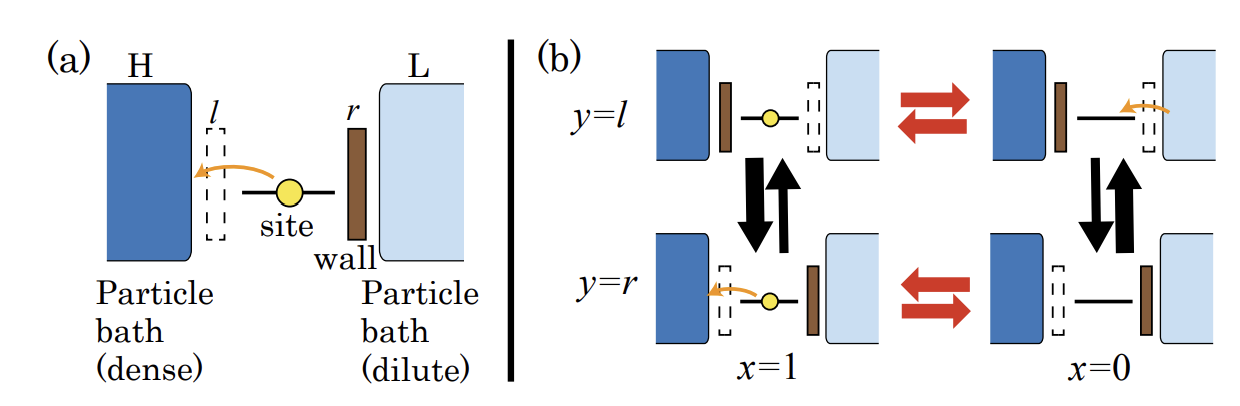
\includegraphics[width=100mm]{4state.png}
    \end{center}
    \caption{4状態モデル}
    \label{fig:4state}
\end{figure}

図のように、化学ポテンシャル$\mu_L$をもつ粒子浴Lから、化学ポテンシャル$\mu_H$をもつ粒子浴Hに粒子が移動する等温過程を考える。ただし、$\mu_H > \mu_L$である。
二つの粒子浴の間にはsiteがあり、最大1個の粒子まで保持することができる。\\
$x \in \{0,1\}$をsiteに粒子があるかないかを表す変数とする。加えて、siteと粒子浴の間には壁を挿入することができ、これがdemonの操作に対応する。壁の位置を$y \in \{l,r\}$で表す。\\
もし、$y =l$であったら、粒子はsiteと粒子浴Hの間を移動できない。同様に、$y = r$であったら、粒子はsiteと粒子浴Lの間を移動できない。そうでないときは、粒子は以下のような遷移確率で遷移可能である。

\begin{align}
    \ln \frac{P_{(r,0) \to (r,1)}}{P_{(r,1) \to (r,0)}} &= \beta \mu_H \\
    \ln \frac{P_{(l,0) \to (l,1)}}{P_{(l,1) \to (l,0)}} &= \beta \mu_L 
\end{align}
%TODOこの式どこからきたか後で確認する。
壁の遷移確率は以下で表されると仮定する:
\begin{align}
    \ln \frac{P_{(r,0) \to (l,0)}}{P_{(l,0) \to (r,0)}} &= \beta E_0 \\
    \ln \frac{P_{(r,1) \to (l,1)}}{P_{(l,1) \to (r,1)}} &= \beta E_1 
\end{align}
ただし、$E_0 > E_1$である。%TODO: ここをもう少し詳しく書く
粒子がsiteに存在するとき壁は右側に(すなわち、粒子がHに入るように)動きやすく、粒子がsiteに存在しないときは、壁は左側に(すなわち、粒子がLに入るように)動きやすい。このようにして、化学ポテンシャルのより高いところに粒子が集められることとなる。\\


\subsubsection{一般の第二法則}
自律的なMaxwell demonについては、沙川-上田関係を用いることはできない。というのも、沙川上田関係では、片方の系を固定して考えていたが、実際にはそんなことはなく、両方時間発展するからである。自律的なMaxwell demonに用いることのできる第二法則のような関係は、以下のようになる。
\begin{align}
    \hat{\sigma}_x(t) \geq \sum_{x,x',y} J^y_{x,x'}(t) \left( \hat{I}_t(x'; y) - \hat{I}_t(x; y) \right). \tag{9.44}
\end{align}
ここで、\(J^y_{x,x'}(t) := J((x', y) \to (x, y); t)\) は時刻 \(t\) における状態 \((x', y)\) から \((x, y)\) への確率流であり、\(\hat{I}_t\) は時刻 \(t\) における確率相互情報である。右辺は情報流と呼ばれ、$X$のカレントにより相互情報量がどれほど変化するかを表す。\\
この関係式は9.5節で導出される。\\

\subsubsection{沙川-上田関係の限界}
上と同じようなことが書いてある。\\

\subsection{部分エントロピー生成およびIFT}
沙川-上田関係においては、系全体のエントロピー生成を部分系に分解することができた。この節では、更に分解して、1つの遷移によるエントロピー生成について考える。\\
\subsubsection{部分エントロピー生成}
時間$0 \leq t \leq \tau$において、状態$w_1, w_2, \cdots, w_M$に対するMarkovジャンプ過程を考える。また、この節では詳細つり合い条件が成り立っているものと仮定する。全系のエントロピー生成
\begin{align}
    \hat{\sigma} = -\sum_{\nu} \beta_{\nu} \hat{Q}_{\nu} + \hat{s}(w(\tau); \tau) - \hat{s}(w(0); 0)
\end{align}
を、それぞれの単一遷移$w' \to w$によるエントロピー生成$\hat{\sigma}_{w' \to w}$に分解する。この分解したあとの$\hat{\sigma}_{w' \to w}$を部分エントロピー生成と呼ぶ。部分エントロピー生成が満たすべき性質として、以下の2つが期待される。
\begin{enumerate}
    \item \textbf{加法性}\\
    任意の一つの経路について、任意の取りうる経路の部分エントロピー生成の和が全系のエントロピー生成になる:
    \begin{align}
        \sum_{w'\to w\in G} \hat{\sigma}_{w' \to w} = \hat{\sigma}
    \end{align}
    ただし、$G$は全ての経路の集合である。
    \item \textbf{IFT}\\
    取りうる経路の集合の、任意の部分集合$\Omega$について、この部分集合の部分エントロピー生成は、
    \begin{align}
        \hat{\sigma}_{\Omega} = \sum_{w' \to w \in \Omega} \hat{\sigma}_{w' \to w}
    \end{align}
    となる。これが、IFT型の等式を満たす:
    \begin{align}
        \ev{e^{-\hat{\sigma}_{\Omega}}} = 1
    \end{align}
\end{enumerate}
\begin{figure}[H]
    \begin{center}
    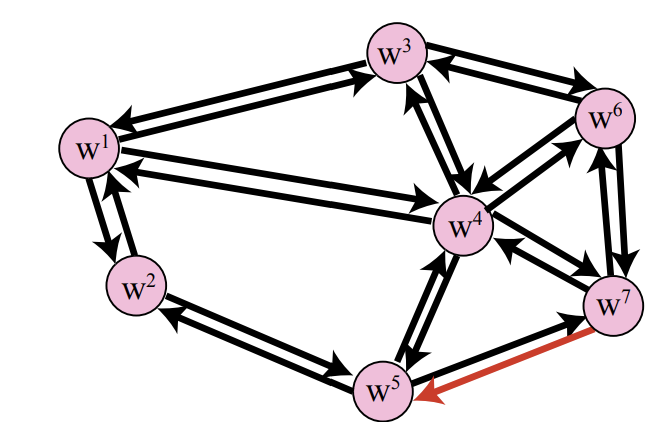
\includegraphics[width=80mm]{partial1.png}
    \end{center}
    \caption{状態空間の例と単一の遷移の選びかた}
    \label{fig:状態空間の例と単一の遷移の選びかた}
\end{figure}

\begin{figure}[H]
    \begin{center}
    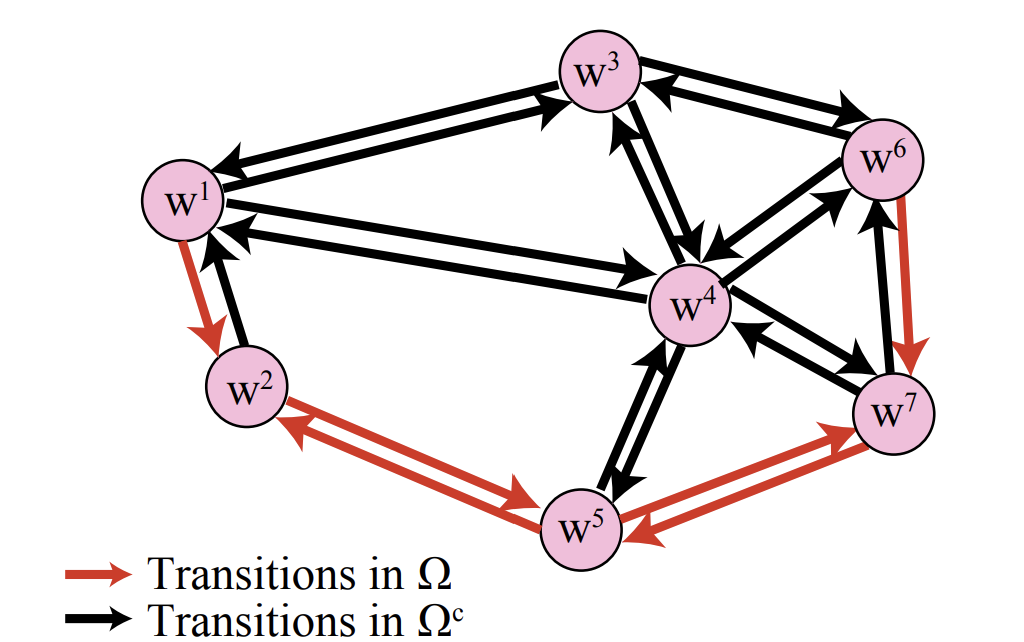
\includegraphics[width=100mm]{ome.png}
    \end{center}
    \caption{部分集合$\Omega$の例}
    \label{fig:ome}
\end{figure}

一つの遷移に対するエントロピー生成を、
\begin{align}
    \hat{\sigma}_{w' \to w} = \beta \hat{Q}_{w' \to w} + \Delta \hat{s}_{w' \to w}
\end{align}
とする。ここで、
\begin{align}
    \delta_{w(t),w} 
    = \begin{cases}
        1 & (w(t) = w) \\
        0 & (w(t) \neq w)
    \end{cases}
\end{align}
とし、
\begin{align}
    \delta_{w' \to w}(w^{(i-1)}, w^{(i)}) = \delta_{w^{(i-1)}, w'} \delta_{w^{(i)}, w}
\end{align}
とする。(すなわち、遷移の順番まできっちり決定するクロネッカーデルタである。)このとき、
\begin{align}
    \hat{Q}_{w' \to w} = \sum_{i = 1}^{N} \hat{Q}_{w^{(i-1)} \to w^{(i)};t^i}\delta_{w'\to w}(w^{(i-1)}, w^{(i)})
\end{align}
となる。$\Delta s_{w' \to w}$は、もう少し定義が複雑である。\\

\begin{figure}[H]
    \begin{center}
    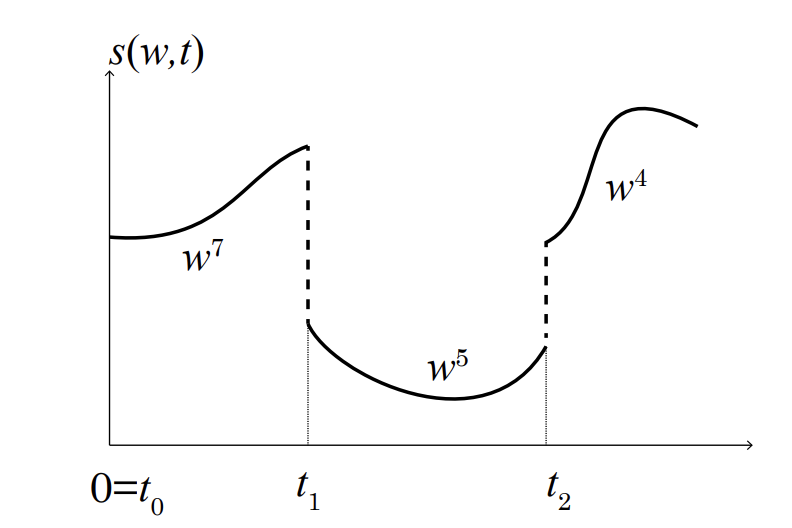
\includegraphics[width=100mm]{stoen.png}
    \end{center}
    \caption{自己情報量の振る舞い}
    \label{fig:one}
\end{figure}

ジャンプによる直接的な自己情報量の変化(離散的)と、ジャンプ後の、確率分布の連続的な変化による自己情報量の変化(連続的)に分けて考える。ジャンプによる自己情報量の変化は、
\begin{align}
    \hat{s}_{w' \to w,\text{jump}} = \sum_{i=1}^{N} (s_{w^{(i)};t^i} - s_{w^{(i-1)};t^i})\delta_{w'\to w}(w^{(i-1)}, w^{(i)})
\end{align}
となる。連続的なほうについて、自己情報量を微分すると、
\begin{align}
    \dv{\hat{s}_{w,t}}{t} &= -\frac{1}{p(w,t)}\dv{p(w,t)}{t}\\
    &= -\frac{1}{p(w,t)}\sum_{w''} J_{w'' \to w; t}\\
\end{align}
となる。ただし、
\begin{align}
    J_{w'' \to w; t} = p_{w'' ,t} P_{w'' \to w; t}- p_{w,t} P_{w \to w''; t}
\end{align}
である。(マスター方程式を思い出すと良い。)これを用いると、$w' \to w$における連続的な部分エントロピー生成は、
\begin{align}
    \hat{s}_{w' \to w, \text{cont}} = -\int_{0}^{\tau} dt \frac{J_{w' \to w; t}\delta_{w(t), w}}{p(w(t), t)}
\end{align}
となる。以上より、エントロピーの変化分は、
\begin{align}
    \Delta \hat{s}_{w' \to w} &= \hat{s}_{w' \to w, \text{jump}} + \hat{s}_{w' \to w, \text{cont}}\\
    &= \sum_{i=1}^{N} (s_{w^{(i)};t^i} - s_{w^{(i-1)};t^i})\delta_{w'\to w}(w^{(i-1)}, w^{(i)}) -\int_{0}^{\tau} dt \frac{J_{w' \to w; t}\delta_{w(t), w}}{p(w(t), t)}
\end{align}
となる。\\

\begin{itembox}[l]{\textbf{Def:部分エントロピー生成}}
    ある単一の$w' \to w$なる遷移について、部分エントロピー生成を、
    \begin{align}
        \hat{\sigma}_{w' \to w} = \beta \hat{Q}_{w' \to w} + \Delta \hat{s}_{w' \to w}
    \end{align}
    と定義する。ただし、
    \begin{align}
        \hat{Q}_{w' \to w} = \sum_{i = 1}^{N} \hat{Q}_{w^{(i-1)} \to w^{(i)};t^i}\delta_{w'\to w}(w^{(i-1)}, w^{(i)})
    \end{align}
    \begin{align}
        \Delta \hat{s}_{w' \to w} = \sum_{i=1}^{N} (s_{w^{(i)};t^i} - s_{w^{(i-1)};t^i})\delta_{w'\to w}(w^{(i-1)}, w^{(i)}) -\int_{0}^{\tau} dt \frac{J_{w' \to w; t}\delta_{w(t), w}}{p(w(t), t)}
    \end{align}
    である。また、遷移の部分集合$\Omega$の部分エントロピー生成は、単一遷移のエントロピー生成を$\Omega$にわたって足し合わせたものとして定義する:
    \begin{align}
        \hat{\sigma}_{\Omega} &= \sum_{w' \to w \in \Omega} \hat{\sigma}_{w' \to w}\\
        &= \beta\hat{Q}_{\Omega} + \Delta \hat{s}_{\Omega}
    \end{align}

\end{itembox}
ここで、以下の四つの式を定義した:
\begin{align}
    \hat{Q}_\Omega &:= \sum_{w' \to w \in \Omega} \hat{Q}_{w' \to w} \\
    \Delta \hat{s}_\Omega &:= \hat{s}_{\Omega, \text{jump}} - \int_0^\tau \frac{J_\Omega(w, t) \delta_{w(t), w}}{p_{w,t}} dt\\
    \hat{s}_{\Omega, \text{jump}} &:= \sum_{w' \to w \in \Omega} \hat{s}_{w' \to w, \text{jump}} \\
    J_\Omega(w, t) &:= \sum_{\{w' | (w' \to w) \in \Omega\}} J_{w' \to w; t}
\end{align}

\subsubsection{部分エントロピー生成に対するIFT}
上で定義した部分エントロピー生成が要請を満たすことを確かめる。\\
\textbf{加法性}\\
定義から、部分エントロピー生成は以下の加法性を満たす:%TODOあとで確認する
\begin{align}
    \hat{\sigma}_{\Omega} = \sum_{w' \to w \in G} \hat{\sigma}_{w' \to w}
\end{align}

\textbf{IFT}\\
\begin{itembox}[l]{\textbf{Thm:部分エントロピー生成に対するIFT}}
    部分エントロピー生成に対して、以下が成り立つ:\footnote{この期待値の経路積分は、$\Omega$と$\Omega^c$の両方の経路積分を含む。}
    \begin{align}
        \ev{e^{-\hat{\sigma}_{\text{tot}}}} = 1
    \end{align}
\end{itembox}
\textbf{Prf}\\
以下のように、遷移行列$P'$を定義する:
\begin{align}
    P'_{w \to w'; t} 
    \begin{cases}
        P_{w \to w'; t} & (w' \to w \in \Omega) \\
        \frac{p_{w',t}P_{w' \to w; t}}{p_{w,t}} & (w' \to w \notin \Omega)
    \end{cases}
\end{align}
これのエスケープレートを計算すると、
\begin{align}
    e'_{w,t} &= \sum_{w'} P'_{w \to w'; t} \\
    &= \left( \sum_{w' : w' \to w \notin \Omega} \frac{p_{w',t}P_{w' \to w; t}}{p_{w,t}}\right) + \left(\sum_{w' : w' \to w \in \Omega} P_{w \to w'; t} \right) \\
    &= \left( \sum_{w' : w' \to w \notin \Omega} P_{w \to w'; t} +\frac{p_{w',t}P_{w' \to w; t}-p_{w,t}P_{w \to w'; t}}{p_{w,t}}\right) + \left(\sum_{w' : w' \to w \in \Omega} P_{w \to w'; t} \right) \\
    &= e_{w,t} + \frac{J_{\Omega^c}(w,t)}{p_{w,t}} 
\end{align}
となる。ここで、$\Omega^c$は$\Omega$の補集合である。\\
つぎに、$e^{-\hat{\sigma}_\Omega}$の寄与を計算する。$w' \to w \in \Omega$について、
\begin{align}
    &P_{w' \to w; t} e^{-\beta \hat{Q}_{\Omega}-\hat{s}_{\Omega, \text{jump}}} = P_{w' \to w; t} \cdot \frac{P_{w \to w'; t}}{P_{w' \to w; t}} \cdot \frac{p_{w,t}}{p_{w',t}} \quad \because \text{自己情報量と熱の定義} \\
    &= P'_{w \to w'; t} \cdot \frac{p_{w,t}}{p_{w',t}} \quad \because \text{$P'$の定義} 
\end{align}
となる。$w' \to w \notin \Omega$については、
\begin{align}
    &P_{w' \to w; t} e^{-\beta \hat{Q}_{\Omega}-\hat{s}_{\Omega, \text{jump}}} \\
    &= P_{w' \to w; t} \cdot 1\quad \because \text{経路$w' \to w$が$\Omega$に含まれない} \\
    &= \frac{p_{w,t}P'_{w \to w'; t}}{p_{w',t}} \quad \because \text{$P'$の定義}
\end{align}
となる。したがって、任意の$w' \to w$について、
\begin{align}
    P_{w' \to w; t} e^{-\beta \hat{Q}_{\Omega}-\hat{s}_{\Omega, \text{jump}}} = P'_{w \to w'; t} \cdot \frac{p_{w,t}}{p_{w',t}}
\end{align}
となる。また、
\begin{align}
    \frac{J_{\Omega}(w,t)}{p_{w,t}} + \frac{J_{\Omega^c}(w,t)}{p_{w,t}} = \frac{1}{p_{w,t}} \dv{t} p_{w,t} = \dv{t} \ln p_{w,t}
\end{align}
である。これより、
\begin{align}
    &\exp(\sum_{w }\int_{0}^{\tau} \dd{t} \frac{J_{\Omega}(w,t)\delta_{w(t), w}}{p_{w,t}}) \\
    &= \prod_{i=0}^{N} \exp(\int_{t^i}^{t^{i+1}} \dd{t} \frac{J_{\Omega}(w^{i},t)}{p_{w^{i},t}}) \\
    &= \prod_{i=0}^{N} \frac{p_{w^{i},t^{i+1}}}{p_{w^{i},t^{i}}} \exp(-\int_{t^i}^{t^{i+1}} \dd{t} \frac{J_{\Omega^c}(w^{i},t)}{p_{w^{i},t}}) \quad \because \text{上で示した等式、積分実行} 
\end{align}
となる。以上の関係より、
\begin{align}
    \ev{e^{-\hat{\sigma}_\Omega}} &= \ev{\exp(-\beta \hat{Q}_\Omega -  \hat{s}_{\Omega,\text{jump}} + \int_{0}^{\tau} \dd{t} \frac{J_{\Omega}(w,t)\delta_{w(t), w}}{p_{w,t}})} \\
    &= \int \dd \Gamma p_{w^{0},0} \cdot \left(\prod_{i=0}^{N} P_{w^{i-1} \to w^{i}; t^i} \right) \cdot \left(\prod_{i=0}^{N} \exp(-\int_{t^i}^{t^{i+1}} \dd{t} e_{w^{i},t}) \right) \\
    &\quad \cdot \exp\left(-\beta \hat{Q}_\Omega -  \hat{s}_{\Omega,\text{jump}} + \int_{0}^{\tau} \dd{t} \frac{J_{\Omega}(w,t)\delta_{w(t), w}}{p_{w,t}} \right) \\
    &= \int \dd \Gamma p_{w^{0},0} \cdot \left(\prod_{i=1}^{N} \frac{p_{w^{i},t^{i}}}{p_{w^{i-1},t^{i}}} P'_{w^{i} \to w^{i-1}; t^i} \right) \cdot \left(\prod_{i=0}^{N} \exp(-\int_{t^i}^{t^{i+1}} \dd{t} e_{w^{i},t}) \right) \\
    &\quad \cdot \left(\prod_{i=0}^{N} \frac{p_{w^{i},t^{i+1}}}{p_{w^{i},t^{i}}} \exp(-\int_{t^i}^{t^{i+1}} \dd{t} \frac{J_{\Omega^c}(w^{i},t)}{p_{w^{i},t}}) \right) \\
    &= \int \dd \Gamma p_{w^{N},\tau} \cdot \left(\prod_{i=1}^{N} P'_{w^{i} \to w^{i-1}; t^i} \right) \cdot \left(\prod_{i=0}^{N} \exp(-\int_{t^i}^{t^{i+1}} \dd{t} e'_{w^{i},t}) \right) \\
    &=\int \dd \Gamma P'(\Gamma^{\dagger})\\
    &= 1
\end{align}

\subsubsection{一般的な情報過程におけるゆらぎの定理}
9.4で述べた通り、沙川上田関係では、自律的なMaxwell demonに対しては適用できない。ここでは、そのような系も扱えるような、一般性のある情報過程に対するゆらぎの定理を述べる。\\
\textbf{設定/記法}\\
\begin{itemize}
    \item 系$X$と$Y$の複合系を考える。
    \item 系$X$がとる状態を$x$、系$Y$がとる状態を$y$とする。
    \item $x \in S_X$、$y \in S_Y$とする。
    \item 時間$0 \leq t \leq \tau$を考え、この間、自身の状態を同時に変化させることはできないとする。
    \item エントロピー生成の定義は沙川-上田関係のものと同様に定義する。すなわち、
    \begin{align}
        \hat{\sigma}_X = \beta\hat{Q}_X + s(x_{N}; \tau) - s(x_0; 0) 
    \end{align}
    である。
    \item それぞれの経路について、jumpの回数を$N$とし、$i$回目のjumpでは、時刻$t = t^i$において状態が$(x^{i-1}, y^{i-1})$から$(x^{i}, y^{i})$に変化するとする。
\end{itemize}
ここで、$x$に関係する相互情報量の変化を定義すると、
\begin{align}
    \Delta \hat{I}_X = \hat{I}_{X,\text{jump}} + \int_{0}^{\tau} \dd t F_X(x(t), y(t), t)
\end{align}
ここで、第1項は、ジャンプによる相互情報量の変化を表しており、
\begin{align}
    \hat{I}_{X,\text{jump}} = \sum_{i=1}^{N} I(x^{i}; y^{i}) - I(x^{i-1}; y^{i-1})\delta_{y^{i-1}, y^{i}}
\end{align}
である。第二項は時間発展による相互情報量の変化を表す。$F$の関数形を決めるために、相互情報量の時間微分を考える。\\
\begin{align}
    \hat{I}_t(x,y) &= \ln \frac{p_{x,y}}{(\sum_{y' \in S_Y} p_{x,y'})(\sum_{x' \in S_X} p_{x',y})} 
\end{align}
とすると、\footnote{略記のため、$p_{x,y}$は$P(x,y)$のことを指す。}
\begin{align}
    \dv{t} \hat{I}_t(x,y) &= \sum_{c \in S_X} \sum_{d \in S_Y} \pdv{\hat{I}_t(x,y)}{p_{c,d}} \dv{p_{c,d}}{t} \\
    &= \sum_{c \in S_X} \sum_{d \in S_Y} \pdv{\hat{I}_t(x,y)}{p_{c,d}} \cdot \left( \sum_{x'} J_{x' ,c}^d(t) + \sum_{y'} J_{y',d}^c(t) \right) 
\end{align}
となる。ここで、
\begin{align}
    J_{x',x}^y(t) = J((x',y) \to (x,y); t) 
\end{align}
である。(上付きの状態を固定して、下付きの状態が遷移を表す。)これの第一項を$F_X(x,y,t)$とすると、
\begin{align}
    F_X(x,y,t) &= \sum_{c \in S_X} \sum_{d \in S_Y} \pdv{\hat{I}_t(x,y)}{p_{c,d}} \cdot \left( \sum_{x'} J_{x' ,c}^d(t) \right) \\
    &= \frac{1}{P(x,y,t)} \sum_{x'} J_{x',x}^y(t) - \frac{1}{P(x,t)} \sum_{y,x'} J_{x',x}^y(t) \label{eq:FX}
\end{align}
となる。\\
$(\because)$((\ref{eq:FX})の導出)\\
\begin{align}
    &\sum_{c\in S_X} \sum_{d \in S_Y} \pdv{\hat{I}_t(x,y)}{p_{c,d}} \cdot \left( \sum_{x'} J_{x' ,c}^d(t) \right)\\
    &= \sum_{c\in S_X} \sum_{d \in S_Y} \pdv{p_{c,d}}\left( \ln \frac{p_{x,y}}{(\sum_{y'' \in S_Y} p_{x,y''})(\sum_{x'' \in S_X} p_{x'',y})} \right) \cdot \left( \sum_{x'} J_{x' ,c}^d(t) \right)
\end{align}
となる。ここで、微分を三つに分けて実行する。対数の分子の部分について、
\begin{align}
    \sum_{c\in S_X} \sum_{d \in S_Y} \pdv{p_{c,d}}\left( \ln p_{x,y} \right) \cdot \left( \sum_{x'} J_{x' ,c}^d(t) \right) &= \frac{1}{p_{x,y}} \sum_{x'} J_{x' ,x}^y(t)
\end{align}
となる。対数の分母の左側について、
\begin{align}
    &\sum_{c\in S_X} \sum_{d \in S_Y} \left(-\pdv{p_{c,d}}\left( \ln \sum_{y'' \in S_Y} p_{x,y''} \right) \right) \cdot \left( \sum_{x'} J_{x' ,c}^d(t) \right) \\
    &= -\sum_{y'' \in S_Y} \frac{1}{p_{x,y''}} \sum_{x'} J_{x' ,x}^{y''}(t)
\end{align}
となる。対数の分母の右側について、
\begin{align}
    &\sum_{c\in S_X} \sum_{d \in S_Y} \left(-\pdv{p_{c,d}}\left( \ln \sum_{x'' \in S_X} p_{x'',y} \right) \right) \cdot \left( \sum_{x'} J_{x' ,c}^d(t) \right) \\
    &= -\sum_{x'' \in S_X} \frac{1}{p_{x'',y}} \sum_{x'} J_{x' ,x''}^{y}(t)
\end{align}
となる。ところで、最後の式の$J$は和をとると$0$になる。(確率の保存)したがって、(\ref{eq:FX})が成り立つ。\hfill\qedsymbol\\

以上の結果を用いて、以下の定理を示す。
\begin{itembox}[l]{\textbf{Thm:一般の情報過程におけるIFT}}
    複合系$X$と$Y$の情報過程に対して、以下が成り立つ:
    \begin{align}
        \ev{e^{-\hat{\sigma}_X + \Delta \hat{I}_X}} = 1
    \end{align}
\end{itembox}
\textbf{Prf}\\

\begin{figure}[H]
    \begin{center}
    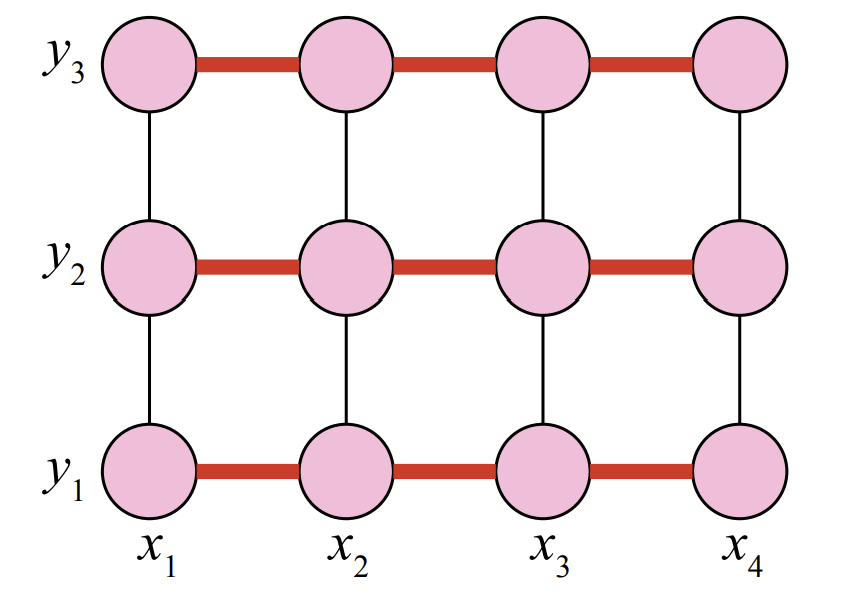
\includegraphics[width=80mm]{omega.png}
    \end{center}
    \caption{$\Omega$の選び方}
    \label{fig:omega}
\end{figure}

$\Omega$を図のように、$X$に関するすべての遷移を含むように選ぶ。このとき、
\begin{align}
    \hat{Q}_{\Omega} &= \hat{Q}_{X}, \\
    \int_{0}^{\tau} \frac{J_{\Omega}(w,t) \delta_{w(t),w}}{p_{w,t}} dt &= \int_{0}^{\tau} \frac{\sum_{x'} J_{x',x(t)}^{y(t)}(t)}{P(x(t), y(t), t)} dt,
\end{align}
である。また、
\begin{align}
    \hat{I}_{X,\text{jump}} &= \sum_{i=1}^{N} \left(\hat{I}_{t^i}(x^{i}, y^{i}) - \hat{I}_{t^i}(x^{i-1}, y^{i-1})\right)\delta_{y^{i-1}, y^{i}} \\
    &= \sum_{i=1}^{N} \left(\log \frac{P(x^{i}, y^{i})}{P(x^{i})P(y^{i})} - \log \frac{P(x^{i-1}, y^{i-1})}{P(x^{i-1})P(y^{i-1})}\right)\delta_{y^{i-1}, y^{i}} \\
    &\text{とくに、$\Omega$に含まれる遷移については、}\\
    &= \sum_{i=1}^{N} \left(\log P(x^{i}, y^{i}) - \log P(x^{i-1}, y^{i}) - \log P(x^{i}) + \log P(x^{i-1}) \right)\\
    &= -\sum_{w' \to w \in \Omega} \hat{s}_{w' \to w, \text{jump}} + \sum_{i=1}^{N} (\hat{s}_{x^{i}, t^i} - \hat{s}_{x^{i-1}, t^i})
\end{align}
である。よって、
\begin{align}
    -\sum_{w' \to w \in \Omega} (\hat{s}_{w' \to w, \text{jump}} ) &= \hat{I}_{X,\text{jump}} -\sum_{i=1}^{N} (\hat{s}_{x^{i}, t^i} - \hat{s}_{x^{i-1}, t^i})\\
    &= \hat{I}_{X,\text{jump}} - \Delta \hat{s}_{X}\\
    &= \hat{I}_{X,\text{jump}} - \hat{s}_{x_N, \tau} + \hat{s}_{x_0, 0} + \int_{0}^{\tau} \sum_{y,x'} \frac{J_{x',x(t)}^{y(t)}(t)}{P(x(t), t)} dt
\end{align}
となる。以上より、%TODOこの下の式の導出あやしい
\begin{align}
    \hat{\sigma}_{\Omega} &= \beta \hat{Q}_{\Omega} + \Delta \hat{s}_{\Omega} \\
    &= \beta \hat{Q}_{X} + \hat{s}_{\Omega, \text{jump}} - \int_{0}^{\tau} \frac{\sum_{x'} J_{x',x(t)}^{y(t)}(t)}{P(x(t), y(t), t)} dt \\
    &= \beta \hat{Q}_{X} - \hat{I}_{X,\text{jump}} + s(x_{N}; \tau) - s(x_0; 0) - \int_{0}^{\tau} \frac{\sum_{y,x'} J_{x',x(t)}^{y}(t)}{P(x(t), t)} dt -\int_{0}^{\tau} \frac{\sum_{x'} J_{x',x(t)}^{y(t)}(t)}{P(x(t), y(t), t)} dt\\
    &= \beta \hat{Q}_{X} - \hat{I}_{X,\text{jump}} + s(x_{N}; \tau) - s(x_0; 0) - \int_{0}^{\tau} F_X(x(t), y(t), t) dt\\
    &= \hat{\sigma}_X - \Delta \hat{I}_X
\end{align}
となる。これと部分エントロピー生成に対するIFTを用いると、
\begin{align}
    \ev{e^{-\hat{\sigma}_X + \Delta \hat{I}_X}} = 1
\end{align}
となる。\hfill\qedsymbol\\

\begin{itembox}[l]{\textbf{Prop:第二法則}}
上のIFTを変形することにより、第二法則が導かれる。すなわち、
\begin{align}
    \dot{\sigma}_x(t) \geq \sum_{x,x',y} J^y_{x,x'}(t) \left( \hat{I}_t(x'; y) - \hat{I}_t(x; y) \right). \tag{9.44}
\end{align}
が成り立つ。
\end{itembox}
\textbf{Prf}\\
Jensenの不等式を用いることで、
\begin{align}
    \ev{e^{-\hat{\sigma}_X + \Delta \hat{I}_X}} \geq e^{-\ev{\hat{\sigma}_X} + \ev{\Delta \hat{I}_X}}
\end{align}
となる。したがって、
\begin{align}
    \ev{\hat{\sigma}_X} \geq  \ev{\Delta \hat{I}_X}
\end{align}
となる。ここで、右辺について、
\begin{align}
    \ev{\Delta \hat{I}_X} &= \ev{\hat{I}_{X,\text{jump}} + \int_{0}^{\tau} \dd t F_X(x(t), y(t), t)} \\
    &\because \ev{F_X(x(t), y(t), t)} = 0\\
    &= \ev{\hat{I}_{X,\text{jump}}}\notag\\
    &= \ev{\sum_{i=1}^{N} \hat{I}(x^{i}; y^{i}) - \hat{I}(x^{i-1}; y^{i-1})\delta_{y^{i-1}, y^{i}}}\\
    &\because \text{今$y$固定しているので}\notag\\
    &= \sum_{i=1}^{N} \ev{\hat{I}(x^{i}; y^{i}) - \hat{I}(x^{i-1}; y^{i})}
\end{align}
となる。したがって、両辺時間微分することで、
\begin{equation}
    \begin{aligned}
    \dv{\ev{\Delta \hat{I}_X}}{t}&=\sum_{x,x',y} \frac{\dd P(x,y,t)}{\dd t} (\sum_{i=1}^{N} \hat{I}(x^{i}; y^{i}) - \hat{I}(x^{i-1}; y^{i}))\\
    &= \sum_{x,x',y}\hat{J}^y_{x,x'}(t) \left( \hat{I}_t(x'; y) - \hat{I}_t(x; y) \right)
\end{aligned}
\end{equation}
となる。以上より、
\begin{align}
    \ev{\hat{\sigma}_X} \geq \sum_{x,x',y} J^y_{x,x'}(t) \left( \hat{I}_t(x'; y) - \hat{I}_t(x; y) \right)
\end{align}
となる。\hfill\qedsymbol\\ %TODO 上の和の取り方についてもう少し考える

 \( \ev{F_X(x, y, t)} \) がゼロであるにもかかわらず、IFT型の等式を得るためには \( F_X(x, y, t) \) が不可避である。
4状態モデルを使用してこの事実を数値的に示す。

\begin{figure}[H]
    \begin{center}
    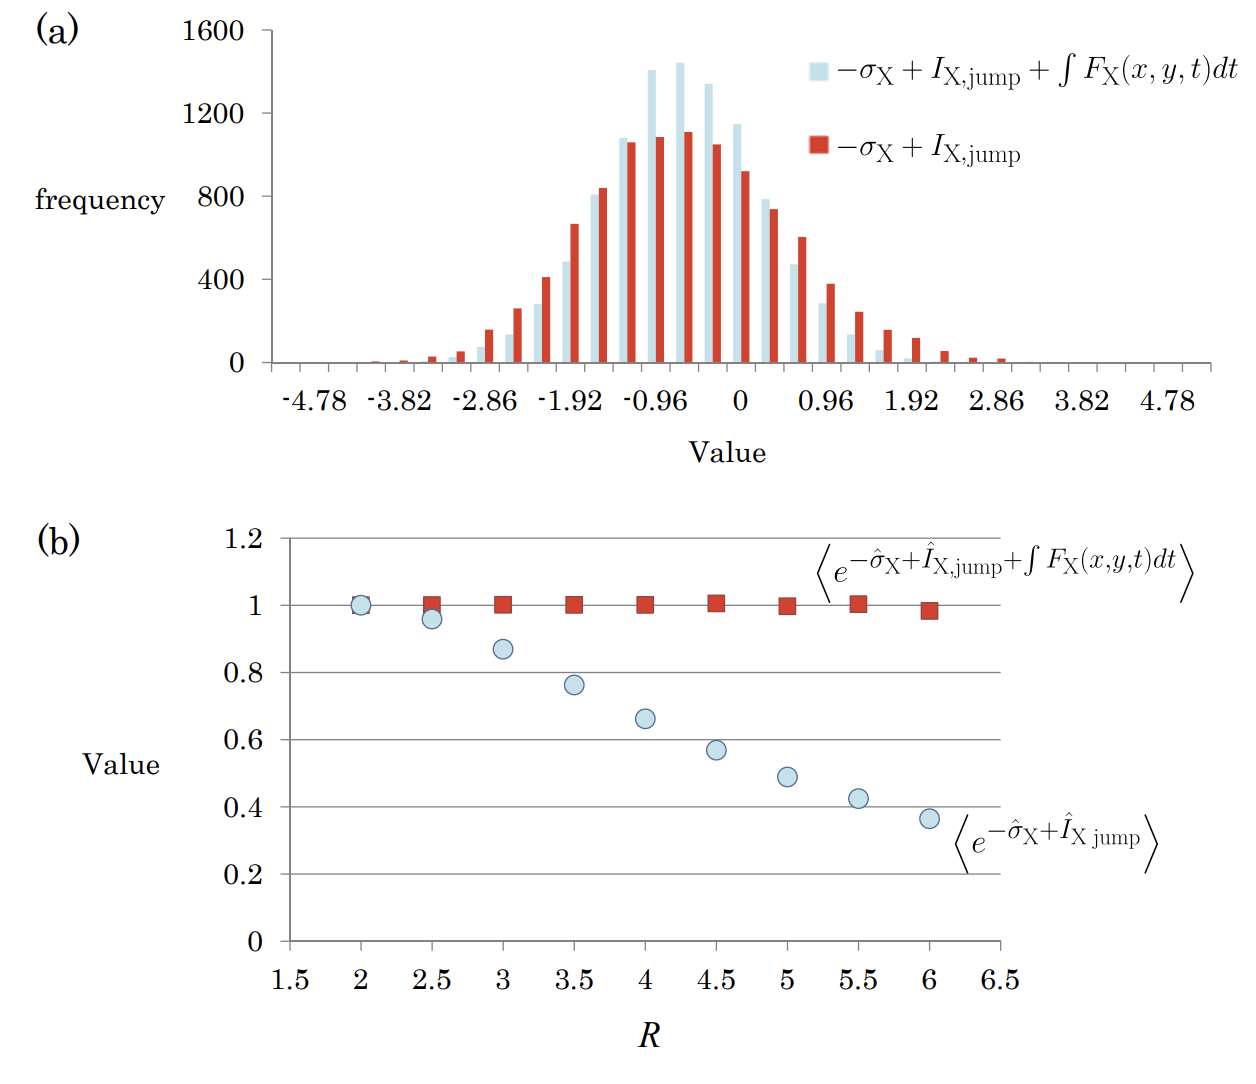
\includegraphics[width=120mm]{4s.png}
    \end{center}
    \caption{4状態モデルの数値計算}
    \label{fig:4s}
\end{figure}

パラメータを以下のように設定する。
\begin{align*}
P(1 \to 0 | r) &= P(0 \to 1 | l) = 1, \\
P(0 \to 1 | r) &= P(1 \to 0 | l) = 2, \\
P(r \to 1 | 1) &= P(1 \to r | 0) = 1, \\
P(1 \to r | 1) &= P(r \to 1 | 0) = R,
\end{align*}
\(\tau = 10\) とし、初期状態を定常状態に設定する。\( R = 3.5 \) のときの \( -\sigma_X + I_{X, \text{jump}} \)(青色)および \( -\sigma_X + I_{X, \text{jump}} + \int F_X(x, y, t) \, dt \)(赤色)の確率分布を計算する。
このヒストグラムからわかるように、\( -\sigma_X + I_{X, \text{jump}} + \int F_X(x, y, t) \, dt \) の分散は \( -\sigma_X + I_{X, \text{jump}} \) よりも大きい。
分布の尾部がIFT型の等式に大きく寄与しているため、\( \langle e^{-\hat{\sigma}_X + \hat{I}_{X, \text{jump}}} \rangle \) は \( R \) が増加するにつれて1から逸脱するが、
\( \langle e^{-\hat{\sigma}_X + \hat{I}_{X, \text{jump}} + \int F_X(x, y, t) \, dt} \rangle \) は1のままである。



\end{document}